\documentclass{pca}


% Overview
% April 12 : 1060 words
% April 13 : 6105 words (cs 7165)
% April 14 : 2624 words
% April 15 : total 11121

\usepackage[T1]{fontenc}
\usepackage{amsthm}
\usepackage{charter}
\usepackage{eulervm}
\usepackage{bbm}
\usepackage[bbgreekl]{mathbbol}
\usepackage[scaled=0.9]{beramono}

\usepackage{amsmath}
\usepackage{amssymb}
\usepackage{graphicx}
\usepackage{svg}
\usepackage{caption}
\usepackage{subcaption}
\usepackage{enumerate}
\usepackage{cancel}
\usepackage{makeidx}
\usepackage{footmisc}
\usepackage{mathrsfs}
\usepackage{float}
\usepackage[many]{tcolorbox}
\usepackage{csquotes}
\usepackage{imakeidx}
\usepackage{booktabs}

\usepackage{alltt}
\usepackage{upquote}
\usepackage{fancyvrb}
\usepackage{mathtools}

\usepackage{listings}

\usepackage{cases}
\usepackage{caption}
\usepackage{geometry}

\usepackage{natbib}
\usepackage{caption}

%\theoremstyle{definition}

%\newtheorem{theorem}{Theorem}

%\newtheorem{definition}{Definition}
%\newtheorem{corollary}{Corollary}
%\newtheorem{lemma}{Lemma}
%\newtheorem{example}{Example}
%\setcounter{tocdepth}{4}
%\floatstyle{ruled}
%\newfloat{pseudo}{h}{lop}
%\floatname{pseudo}{Algorithm}

%\let\doendproof\endproof
%\renewcommand\endproof{~\hfill\qed\doendproof}

\usepackage{color}
\usepackage{xcolor}

\newcommand{\p}{\,\text{.}}

\newenvironment{aside}{
	\setlength{\leftskip}{1em}\par\itshape
}{
	
	\setlength{\leftskip}{0em}\par
}

\definecolor{my-green}{HTML}{677d00}
\definecolor{my-light-green}{HTML}{acd373}
\definecolor{my-lighter-green}{HTML}{e6ecce}
\definecolor{my-red}{HTML}{b13e26}
\definecolor{my-light-red}{HTML}{d38473}
\definecolor{my-blue}{HTML}{306693}
\definecolor{my-light-blue}{HTML}{73a7d3}
\definecolor{my-gray}{HTML}{999999}
\definecolor{my-orange}{HTML}{E69500}
\definecolor{my-light-orange}{HTML}{FFC353}

\usepackage[colorlinks=true,citecolor=my-red,urlcolor=my-green,linkcolor=my-red]{hyperref}

\newcommand{\lgc}[1]{{\color{my-light-green} #1}}
\newcommand{\gc}[1]{{\color{my-green} #1}}
\newcommand{\lrc}[1]{{\color{my-light-red} #1}}
\newcommand{\rc}[1]{{\color{my-red} #1}}
\newcommand{\lbc}[1]{{\color{my-light-blue} #1}}
\newcommand{\bc}[1]{{\color{my-blue} #1}}
\newcommand{\kc}[1]{{\color{my-gray} #1}}
\newcommand{\loc}[1]{{\color{my-light-orange} #1}}
\newcommand{\oc}[1]{{\color{my-orange} #1}}

\newcommand{\mba}{\mathbold a}
\newcommand{\mbA}{\mathbold A}
\newcommand{\mbb}{\mathbold b}
\newcommand{\mbB}{\mathbold B}
\newcommand{\mbc}{\mathbold c}
\newcommand{\mbC}{\mathbold C}
\newcommand{\mbd}{\mathbold d}
\newcommand{\mbD}{\mathbold D}
\newcommand{\mbE}{\mathbold E}
\newcommand{\mbf}{\mathbold f}
\newcommand{\mbg}{\mathbold g}
\newcommand{\mbh}{\mathbold h}
\newcommand{\mbI}{\mathbold I}
\newcommand{\mbK}{\mathbold K}
\newcommand{\mbL}{\mathbold L}
\newcommand{\mbm}{\mathbold m}
\newcommand{\mbM}{\mathbold M}
\newcommand{\mbo}{\mathbold o}
\newcommand{\mbr}{\mathbold r}
\newcommand{\mbs}{\mathbold s}
\newcommand{\mbt}{\mathbold t}
\newcommand{\mbS}{\mathbold S}
\newcommand{\mbz}{\mathbold z}
\newcommand{\mbv}{\mathbold v}
\newcommand{\mbk}{\mathbold k}
\newcommand{\mbp}{\mathbold p}
\newcommand{\mbP}{\mathbold P}
\newcommand{\mbq}{\mathbold q}
\newcommand{\mbQ}{\mathbold Q}
\newcommand{\mbbr}{\mathbold r}
\newcommand{\mbR}{\mathbold R}
\newcommand{\Sig}{\mathbold \Sigma}
\newcommand{\mbft}{\mathbold t}
\newcommand{\mbT}{\mathbold T}
\newcommand{\mbe}{\mathbold e}
\newcommand{\mbu}{\mathbold u}
\newcommand{\mbU}{\mathbold U}
\newcommand{\mbfv}{\mathbold v}
\newcommand{\mbV}{\mathbold V}
\newcommand{\mbw}{\mathbold w}
\newcommand{\mbW}{\mathbold W}
\newcommand{\mbx}{\mathbold x}
\newcommand{\mbX}{\mathbold X}
\newcommand{\mby}{\mathbold y}
\newcommand{\mbY}{\mathbold Y}
\newcommand{\mbfz}{\mathbold z}
\newcommand{\mbZ}{\mathbold Z}

\newcommand{\one}{\mathbold 1}

%\newcommand{\p}{,\text{.}}
\newcommand{\tab}{\hspace{1em}}

\newcommand{\mR}{\mathbb R}
\newcommand{\mE}{\mathbb E}
\newcommand{\mC}{\mathbb C}
\newcommand{\mN}{\mathbb N}
\newcommand{\mV}{\mathbb V}
\newcommand{\mZ}{\mathbb Z}

\newcommand{\kp}{\kc{\partial}}
\newcommand{\slice}[1]{\texttt{#1}}

%\newcommand{\deg}{^{\circ}}

\newcommand{\h}{\hspace{0.2em}}

\newcommand{\argmin}[1]{\underset{#1}{\text{argmin}}}
\newcommand{\argmax}[1]{\underset{#1}{\text{argmax}}}

\setcounter{tocdepth}{1}

% Smaller Hadamard operators
\DeclareMathOperator*{\sotimes}{\text{\raisebox{0.25ex}{\scalebox{0.8}{$\otimes$}}}}
\DeclareMathOperator*{\soplus} {\text{\raisebox{0.25ex}{\scalebox{0.8}{$\oplus$}}}}
\DeclareMathOperator*{\soslash}{\text{\raisebox{0.25ex}{\scalebox{0.8}{$\oslash$}}}}
\DeclareMathOperator*{\sominus}{\text{\raisebox{0.25ex}{\scalebox{0.8}{$\ominus$}}}}


%%% Proofs and theorems %%%

\definecolor{proofcolor}{RGB}{200, 200, 200}
\definecolor{theorembordercolor}{RGB}{151, 63, 5}
\definecolor{theorembackgroundcolor}{RGB}{248, 241, 234}

% table spacing

\setlength{\arrayrulewidth}{0.5mm}
\setlength{\tabcolsep}{18pt}
\renewcommand{\arraystretch}{1.5}

\newtheoremstyle{theorem}
{0pt}{0pt}{\normalfont}{0pt}
{}{}{0em}
{\hspace{-0.33em}\thmnote{\normalfont\bfseries\color{my-green}~#3}\hspace{0.7em}}

\theoremstyle{theorem}

\newtheorem{theorem}{Theorem}
\tcolorboxenvironment{theorem}{
    enhanced jigsaw, pad at break*=0mm, breakable,
    grow to left by=5mm,left*=0mm, grow to right by =5mm, right*=0mm, top=2mm, bottom=2mm,
    colback=my-lighter-green, boxrule=0pt, frame hidden,
    borderline west={1mm}{0mm}{my-green}, arc=.5mm
}

%% Definition %%

\newtheoremstyle{definition}
{0pt}{0pt}{\normalfont}{0pt}
{}{}{0em}
{\hspace{-0.33em}\thmnote{\normalfont\bfseries\color{my-green}~#3}\hspace{0.7em}}

\theoremstyle{definition}

\newtheorem{definition}{Definition}
\tcolorboxenvironment{definition}{
    enhanced jigsaw, pad at break*=0mm, breakable,
    grow to left by=5mm,left*=0mm, grow to right by =5mm, right*=0mm, top=2mm, bottom=2mm,
    colback=my-lighter-green, boxrule=0pt, frame hidden,
    borderline west={1mm}{0mm}{my-green}, arc=.5mm
}

%%  Proof %%%

\makeatletter

\makeatletter

\def\renewtheorem#1{%
    \expandafter\let\csname#1\endcsname\relax
    \expandafter\let\csname c@#1\endcsname\relax
    \gdef\renewtheorem@envname{#1}
    \renewtheorem@secpar
}
\def\renewtheorem@secpar{\@ifnextchar[{\renewtheorem@numberedlike}{\renewtheorem@nonumberedlike}}
\def\renewtheorem@numberedlike[#1]#2{\newtheorem{\renewtheorem@envname}[#1]{#2}}
\def\renewtheorem@nonumberedlike#1{
    \def\renewtheorem@caption{#1}
    \edef\renewtheorem@nowithin{\noexpand\newtheorem{\renewtheorem@envname}{\renewtheorem@caption}}
    \renewtheorem@thirdpar
}
\def\renewtheorem@thirdpar{\@ifnextchar[{\renewtheorem@within}{\renewtheorem@nowithin}}
\def\renewtheorem@within[#1]{\renewtheorem@nowithin[#1]}

\makeatother

\newtheoremstyle{proof}
{0pt}{0pt}{\normalfont}{0pt}
{}{}{1em}
{{\bfseries\color{proofcolor}\thmname{#1}.}
    \thmnote{\normalfont\color{black}~(\textit{#3})}}

\theoremstyle{proof}
\renewtheorem{proof}{Proof}

\tcolorboxenvironment{proof}{
    enhanced jigsaw, pad at break*=0mm, breakable, parbox=false,
	grow to left by=5mm,left*=0mm, grow to right by =5mm, right*=0mm, top=2mm, bottom=2mm, colback=white, boxrule=0pt, frame hidden, before skip=0mm,
    borderline west={1mm}{0mm}{proofcolor}, arc=.5mm
}

\title{embeddings, attention and scale\\ the simplicity of modern machine learning}

\DeclareCaptionFormat{custom}
{%
    \textbf{#1#2}{\setlength{\leftskip}{1em}\par #3\setlength{\leftskip}{0em}\par}
}
\captionsetup{format=custom}


\date{\today}

% non-indented, spaced paragraphs
\setlength{\parindent}{0.0in}
\setlength{\parskip}{0.1in}


\lstdefinestyle{mystyle}{
    commentstyle=\color{gray},
    basicstyle=\ttfamily,
    breakatwhitespace=false,         
    breaklines=true,                 
    captionpos=b,                    
    keepspaces=true,                 
    numbers=left,                    
    numbersep=5pt,                  
    showspaces=false,                
    showstringspaces=false,
    showtabs=false,                  
    tabsize=2
}

\lstset{
	style=mystyle,
	escapeinside={|<}{>|}
}

\makeindex

\begin{document}

\maketitle

\tableofcontents

\chapter*{About this book}

\emph{Machine Learning} is the business of creating computer programs that learn from examples. This is in contrast to more traditional programming where we give the computer a bunch of rules to follow.

A simple example is recognizing written digits. We know that this task can be solved, because we ourselves can solve it. And yet, if you try to compe up with a set of rules for what makes a three a three, you soon find yourself awash in a flood of counterexamples. Things that don't follow the rules you've set, but that are unmistakably threes to any human observer.


The reason we can do this so easily without knowing the rules is that we were never given any rules. All we were given were a bunch of \emph{examples}. Machine learning is the business of trying to make computers grasp concepts---like what a three is---from a set of examples, without any explicit rules. 

When I first studied machine learning, somewhere around 2003, the field was, like artificial intelligence in general, defined by what we couldn't do. We had some simple successes, like early spam detectors, but primarily the feeling was that we hadn't yet cracked it. 

Thus, studying machine learning meant studying a large number of disparate approaches: kernel methods, graphical models, neural models, and so on. Each with their own language, algorithms and textbooks. 

Starting around 2011, neural models, or \emph{Deep Learning} began to show tremendous progress, quickly taking over the field. The other methods were still used, but only to the extent that they could be combined with deep learning. The effect, apart from upsetting many researchers whose eggs were in the wrong basket, was to simplify the field. The language of deep learning has its complexities, but the basics are relatively simple. And even when things do get complex, we at least know which complexities to master, rather than having to choose between many subjects that could each take years to master.

Then, around 2016, \emph{attention models}, a subset of deep learning models, arrived. This simplified things further. In deep learning, we don't worry much about how our models are trained, focusing instead on what the model itself looks like, the architecture. When attention models came along, we found that we could pay increasingly less attention to fitting the architecture to the task. So long as we could make the model large enough, and pump enough data through it, a general architecture was all we needed.

The result is that we now have a hugely simplified view of what machine learning is. Or at least, what a minimal required knowledge is to understand modern machine learning systems. 

In books and courses, hovever, the story is still told chronologically. You first learn classical machine learning first, and then neural models on top of that. From there you progress to deep neural models, and then you are finally ready to start tackling the attention models.

This is a classic pattern of academic teaching. We teach the next generation every single step we took to get from point A to point B. No shortcuts and no simplifications. This is perhaps understandable. There isn't always time to review and simplify course material, and it takes a while before you can be sure that the things you would remove actually won't crop up again.

However, after a while we should face the music, and recognize that to some extent we always take the long way around. If there is a more direct route to the end goal, we should teach that. 

This book is an attempt to do that. To teach the modern, simple language of machine learning, with the historical baggage either removed, or moved out of the way. 


\chapter{Embeddings}

% *** 12 Apr ***

\section{A running example: movie reviews}

Here is a movie review, for the movie ... that was posted to the Internet Movie Database (IMDb) on ... by the user.

\blockquote{}

Would you say this is a \bc{positive} or a \rc{negative} review? It's bit ambiguous, but I'd say that this is more positive than negative. Happily, we can validate our guess, because IMDb asks users to give a rating out of 10 along with the review. In this case, the user gave a rating of .... Assuming that less than 5 is negative and more than 5 is positive, we can assume that our guess was correct.

When we try to make computers perform this task, we call it \emph{sentiment classification}: guessing, usually by looking at a lot of examples, whether the sentiment of a given piece of text is positive or negative. Movie reviews on IMDb are a particularly simple starting point, because the star rating gives us a ground truth to learn from. After we guess, we can look at the star rating, and see how well we did. 

It's also a good place to start with simple models. For instance, the type of model that we will start with in this chapter doesn't see the ordering of the words in the review. It sees \emph{which words} are in the review, but not in which order. That means the model sees something like this:

...

This removes a lot of information, but it still allows us to make a pretty good guess as to whether the review was good or bad. Since these models are so simple, it gives us a good starting point for our journey. We can add complexity to our model bit by bit, and at each point, see how much better the model's guesses get.

\begin{aside}
Guessing whether a movie review is positive or negative may seem a bit pointless, especially if IMDb already ensures that each review comes with an explicit rating. However, the general idea of sentiment classification can be very useful. For instance, if you're a moderator of a social network, seeing which posts or message have negative sentiment can be very useful for detecting the more toxic corners of your community.
\end{aside}

To learn to predict whether a movie review is positive or negative, we need to figure out a way to feed the review to a machine learning model. There are a few strategies for this. The first is to \emph{extract some features}. Turn the string of symbols---whose length varies from one review to another---into a vector of a fixed length. Each element of the vector, each feature, \emph{measures} something about the review: whether the word ``terrible'' occurs in it, how many of the letters are capitalized, that sort of thing. If we go down this route, it's up to us to come up with good features: if we pick the wrong ones, we may lose information vital to the classification task: something that is there in the raw text, but not in the feature vector. 

A key aspect of \emph{deep learning} is to avoid feature extraction. By showing the model the raw data as much as possible, we hope to avoid losing any information that may be important. The ultimate aim is to create a model that \emph{learns} which features to extract from the data, rather than doing it ourselves.

This means that we need to do two things. First, we need to translate the movie review somehow to the language of scalars vectors and matrices, and then, we need to craft a model that can deal with the fact that each review has a different length.

The first decision we will make is to model the review as a sequence. In fact, for about the first half of this book, we will deal purely with \emph{sequence models}.

The next question then, is a sequence of what? We can think of the review as a sequence of \emph{characters}. This is how it's represented in computer memory, so it's in some sense the most raw form of the data. The closest to the ideal of Deep Learning that we can get: if we model our review as a sequence of characters, and figure out a model that can read such a sequence, we give our model all the information we have available.

However, to start with, it's easier to think of our review as a sequence of \emph{words}. That is, to the model, the review looks like this:

...

A sequence of symbols, where each symbol is a complete word. The model may see that the words ``terrible'' and ``terrific'' are both in the sentence, and it may learn that they have opposite sentiments, but it will never be able to see how similar their spellings are.

Seeing our data as a string of words has some downsides: for example if a word is misspelled, our model cannot learn to infer what the author meant to type. For now, we will accept that limitation. The string of words view gives us a decent starting point. We will introduce more powerful and flexible approaches later. 


\section{Embeddings}

The main idea we want to introduce in this chapter is that of the \emph{embedding vector}. This idea solves the following problem: we want to represent a word like ``terrible'' in such a way that our model (however we build it) can learn from its properties. But \emph{we don't know any of its properties}. All we see is, for a given review, whether or not the word ``terrible'' appears in it. 

If we were doing classic machine learning we might be tempted to represent ``terrible'' by a feature vector. We could annotate for each word whether it's a noun, a verb or an adjective, whether its aspect is negative, neutral or positive, how many letters it has, and what page it appears on in the dictionary. If we come up with enough features, maybe we can capture some of the relevant properties for our task.

Again, this is not the philosophy we aspire to in this book. That sort of thing is a lot of work, and we might not even be picking very good features. What we \emph{will} copy from this approach is that we will represent every word by a vector. Here we will introduce our first bit of notation. For the word \emph{terrible}, we will come up with a vector to represent it. We will call this vector

\[
\oc{\mbv}_\text{terrible} \p 
\]

% *** 13 Apr ***

How do we come up with these vectors? As a starting point, let's just fill it with random values. We pick a length $k$ for the vectors (the number of elements each vector contains), and we sample a random value for each element. Perhaps uniformly between $0$ and $1$ or from the standard normal distribution, the details don't matter that much.

\begin{aside}
The value $k$ is a hyperparameter. Depending on what we do with these vectors higher or lower values may be better. We usually choose $k$ by trial and error.	
\end{aside}

You can think of this as assigning random features to an object, for want of actual features. This may seem a little silly, since these random features won't actually express any properties of the object. This is true, but at least they will allow us to tell the different objects \emph{apart}. Each word will have a different vector, so whatever model consumes these vectors can at least learn to do different things depending on what words we give it.

We sample one of these vectors for every word we expect to encounter, before we build our model. This means we need to choose a cutoff point. The number of possible words isn't quite infinite, but if we allow for misspellings, proper nouns and words in another language, the number grow very big very quickly. We don't want to store billions of vectors, especially if most of them are very rare, so we take only the $V$ words that are most frequent in our training data. To keep things concrete, you can imagine we set $V$ to $100\h 000$. These $100\h 000$ words are our \emph{vocabulary}.

For the rest of the words, we create a special vector $\oc{\mbv}_{.\text{.unk}}$ (``unk'' for \emph{unknown}). Every word that is not in our vocabulary, we represent with this special vector. That way we can at least tell our model that there is a word in a certain position, even if we cannot represent the word itself in the same way we represent other words.

With this, we can represent a movie review (with some typos) like 
\begin{quote}
This movie was terrbile. It suched.
\end{quote}

as the sequence of vectors 
\[
\oc{\mbv}_\text{this}, \oc{\mbv}_\text{movie}, \oc{\mbv}_\text{was}, \oc{\mbv}_{.\text{unk}}, \oc{\mbv}_\text{it}, \oc{\mbv}_{.\text{unk}}\p 
\]

We lose the most salient words, but at least we can represent the review.

\begin{aside}
	Note that we've assumed that punctuation is removed, and that all words have been transformed to lowercase. This is definitely removing information that might be relevant, but we'll keep things simple for now.
\end{aside}

Next, we want to take this sequence of representations of words in the review, and combine all these different representations into a single representation (another vector) of the \emph{whole} review. Moreover, we need to do this in a way that allows us to process reviews of different lengths. A simple way to achieve this, is to take the mean of all the vectors in the review. We compute

\[
\mbh = \frac{1}{L} \sum_{w} \oc{\mbv}_w 
\]

where $\mbh$ is the representation of our whole review, and $L$ is the length of the review in words. The sum is over all words $w$ in the review. 

The result $\mbh$ may not yet convey much about the review, since we've just filled each vector with random values, but we will at least get a different $\mbh$ for each review. If we're lucky, this difference already contains some pattern that we can build on to make our prediction.

To keep things simple, we will use a very simple one-layer neural network (or equivalently, logistic regression), to make our prediction from $\mbh$.  We define a vector of weights $\oc{\mbw}$ and a scalar bias $\bc{b}$ and compute
\[
y = \sigma (\oc{\mbw}^T\mbh + \bc{b})
\]

where $\sigma$ represents the logistic sigmoid. This means that $y$ is a value between 0 and 1, so we can interpret it as the probability, according to the model, that the class of this review is \bc{positive}. 

Here is the whole model in a diagram.

--

From here, we proceed as in any classification network. We let $p$ be the model's probability of the correct class. That is $p = y$ if the true class is \bc{positive} and $p = 1 - y$ if the true class is \rc{negative}. We then use the logarithmic loss as the value that we want to minimize
\[
l = - \log p \p 
\]

We achieve this minimization by \emph{gradient descent}. For each parameter of the model, currently $\bc{b}$ and the elements of $\oc{\mbw}$, we compute the derivative of the loss with respect to that parameter. That is, we work out $\kp l / \kp \oc{w}_i$ and $\kp l / \kp \bc{b}$. This is done through backpropagation as explained in Appendix~\ref{}. 

We use the notation $\oc{\mbw}^\nabla$ in this book for the vector consisting of all derivatives of the loss with respect to some element of $\oc{\mbw}$. See the appendix for a detailed definition.

With this, we can start to train our model. We take a review, process it into a sequence of words, map each word to its corresponding vector and average these vectors. We pass the average vector though the neural network layer, get a probability for the class, and backpropagate the loss to update the neural network weights.

So far, we haven't done much more than generate random, likely uninformative features for our review, and pass them through a logistic regression. This is a linear model, so it's unlikely to do particularly well in our randomly generated feature space. Still, if the dimensionality of our vectors ($k$) is high enough, we may get a little separation just by chance. 

Now, however, we apply the big magic trick. One of the three main ideas that will provide the foundation for the modern brand of machine learning that this book dicusses. \textbf{We treat the values of our word vectors $\oc{\mbv}_\_$ as parameters of the model.}

\subsection{From random features to embeddings}

Technically, there is nothing special about what we're going to do. In our random feature model, we had some parameters $\oc{\mbw}$, so to train the model, we computed their derivatives $\oc{\mbw}^\nabla$, and then updated them by gradient descent.

What we do now is simply to give the word vectors $\oc{\mbv}_\_$ the same treatment. Say, for instance, that the word ``terrible'' appeared in the review for which we made a prediction and got a loss $l$. That means we used the vector $\oc{\mbv}_\text{terrible}$ in computing our prediction, and we can thus define the vector 
\[
\oc{\mbv}_\text{terrible}^\nabla \p 
\]
 If $\oc{v}_i$ is the $i$-th element of the vector $\oc{\mbv}_\text{terrible}$, then the $i$-th element of the vector $\oc{\mbv}_\text{terrible}^\nabla$ is the derivative of the loss $l$ with respect to $\oc{v}_i$.
 
 Just like the elements of $\oc{\mbw}^\nabla$, we can work out the elements of $\oc{\mbv}_\text{terrible}^\nabla$ by backpropagation, and let gradient descent update $\oc{\mbv}_\text{terrible}$ for us.
 
 \begin{aside}
 It's instructive to work out what this gradient looks like, to see how the model learns, but we'll save that for later. For now, we just assume that we have an automatic differentiation system like Pytorch in place that can handle this for us.
 \end{aside}
 
 When we update the values of $\oc{\mbv}_\text{terrible}$ in this way, we call $\oc{\mbv}_\text{terrible}$ an \emph{embedding vector} for the word terrible. That is, it embeds the ``meaning'' of the word terrible in the space $\mR^k$
 
 While all this is technically very straightforward, I find that for many people starting out with deep learning, embedding vectors require a certain mental leap to comprehend. I think this is due to two properties.
 
 \paragraph{dynamic computation} When we use embedding vectors, we load different vectors, depending on which words are contained in the input sequence. This is a little unusual, especially when those vectors are treated as parameters of the model. One way of thinking about this is that our model consists of a dynamic computation: different model parameters are loaded and updated for each instance, depending on what the instance looks like.
 
 \paragraph{The interplay between model and features} If we think of embeddings as ``learned features'' this may instantly raise a little red flag in the back of our mind. Isn't that cheating, somehow? For instance if I want to learn whether people in some dataset speak French or English, and I do this on the basis on features I've learned, am I really learning anything? I can just come up with any features, but surely the information I base my guess on must be given, rather than invented?
 
 This is true, and if we replace feature vectors with embedding vectors in classical machine learning, we would indeed see the classic signs of cheating: the training loss would go to zero, and the test loss would be no better than chance level. We would start \emph{overfitting}: memorizing the labels of the instances in our training data in a way that doesn't tell us anything about the labels of the instance in our \emph{test} data. The problem is that we have too much freedom to manipulate how one instance is represented, without it affecting the representation of other instances. For learning that generalizes from the seen instances (the training data) to the unseen instances (the test data) that freedom should somehow be constrained. If I manipulate the features of one instances, some or all of the other instances should change as well.
 
 The difference in our case is that we're not embedding the instances (the movie reviews) themselves, but only the words in them. There is still plenty of given information that we cannot manipulate: which words appear in which review. Moreover, we cannot easily manipulate the representation of one review without it affecting the representation of other reviews. If we change the embedding vector $\oc{\mbv}_\text{terrible}$ to make it more likely that the current model outputs the \bc{positive} class for the current review, then the representation of every other review that contains the word ``terrible'' is also changed. Most likely also making those more likely to be classified as \bc{positive}. 
 
 This is exactly the sort of mechanism we are looking for. Even though we are learning our own ``features'' for the words, each word occurs in multiple reviews, allowing us to make a change to one review that affects all other reviews in which the word occurs. For a neutral word, like ``movie'' which will probably occur in positive and negative reviews about equally often, the representation will get pulled this way and that equally, resulting in the contribution to the classification averaging out into a neutral contribution. In short, knowing that the word ``movie'' occurs in a review doesn't tell us much about the sentiment of the review. For ``terrible'', however, we can expect that most reviews containing the word terrible are negative. Therefore the vector $\oc{\mbv}_\text{terrible}$ will slowly get pushed in a direction that makes the classifier more likely to predict the negative class.
 
 \begin{aside}
 Of course, the word terrible can also occur in positive review. For instance, if the author states that the movie is not terrible, or that it's nothing like some other movie, which was terrible. However, on average, we can probably still say that the presence of the word terrible makes the review more likely to be negative.
 \end{aside}
 
 \section{Implementing embedding vectors}
 
 To understand embedding vectors in detail, it's instructive to see how they are implemented. 
 
 \begin{aside}To keep this book general, we will write all our implementations in pseudocode. We will assume we are working in a tensor-based automatic differentiation system like Pytorch or Tensorflow. In particular, we will adopt the \emph{slicing} syntax from those systems. If you are familiar with either of these systems, this should look very familiar. See the appendix for a detailed definition of our pseudocode. 
 \end{aside}

To start with, we will assume that the training data has been pre-processed, and that a vocabulary of $V$ words has been chosen. Together with the \texttt{.unk} vector, this means we need $V+1$ embedding vectors. We'll assume some mapping has been created between the integers $1 \ldots V+1$ and the words in our vocabulary. That way, each review can be represented by a list of integers. As we noted before, we will---for the moment---remove all punctuation and convert everything to lowercase.

To store our embedding vectors, we create a matrix $\oc{\mbV}$ with size $k$ by $V$. If the word \texttt{terrible} is, say, the 910th word in our vocabulary, then the 910th column of $\oc{\mbV}$, is the embedding vector for ``terrible''. Or, using our slicing syntax
\[
\oc{\mbv}_\text{terrible} = \oc{\mbV}\slice{[:, 910]}
\]

This means that if we have a review $r$ containing the text ``This movie was terrible.'',  we can represent it by an integer sequence like $(51, 179, 67, 910)$. Using our slicing syntax, we can extract the four embedding vectors for the words in r and concatenate them into one matrix $\oc{\mbV}_r$ representing the review
\[
\oc{\mbV}_r = \oc{\mbV}\slice{[:, (51, 179, 67, 910)]} \p 
\]

 % TODO: Replace by actual values

The result is a matrix with $k$ rows and four columns, whose first column is the 51st column of $\oc{\mbV}$, whose second column is the 179th column of $\oc{\mbV}$ and so on.

All that is left to do now, is to average the columns of this matrix, and to feed the resulting vector to a single layer neural net. Put together, the whole procedure looks like this

-- pseudocode
 
To visualize the result, we can train this model with $k=2$. Normally, we would set our embedding dimension much higher, but in such a simple model as this, we don't expect the embeddings to contain much more information that how positive or negative the word is likely to make the review, independently of whatever other words appear. This is a one-dimensional property, so in this case, two dimensions might be enough.

The model converges quickly, and scores a test accuracy of \ldots .

% -- TODO: Document hyperparameters

We can now scatterplot the resulting embedding vectors. Here is the resulting point cloud, with some interesting words highlighted. 

-- Point cloud

% TODO: PLay around, see if you can see some other interesting stuff.
 
\subsection{A note on batching in sequence models}
 
At this point it's worth noting that while the pseudocode for our algorithms is usually presented in a non-batched fashion---looping over individual instances---in practice, you will almost always want to translate this to a \emph{batched} implementation, where the model processes a small number of instances in parallel. This helps to both stabilize and to speed up training.

\begin{aside}
You sometimes have multiple tensors, for instance one for the inputs, and one for the target labels. The more precise requirement is that the number of tensors shouldn't depend on how many instances you have in your batch.	
\end{aside}


In a setting like ours, where each instance is a sequence with a different length, this requires a little care to get right. The key to batching is that all the data in your batch should be in one tensor. This is what helps us compute in parallel in a straightforward manner: we simply define our algorithm in operations on this single tensor, and assume that whoever implemented those operations made sure they were parallelized and offloaded to special hardware like GPUs as much as possible. 

The problem with instances of different sequence lengths is that while we can easily concatenate the embedding vectors for a given review into a matrix, the matrices we get in one batch will have different numbers of columns. This means we cannot easily concatenate them into a single 3-tensor.

-- image

There are many solutions, but the simplest one, which make the fewest assumptions about the structure of the data is \emph{padding}. We simply add one more special token to our vocabulary, in the same vein as \texttt{.unk}. We call this token \texttt{.pad}. It gets its own embedding vector $\oc{\mbv}_\texttt{.pad}$, which brings the total size of our vocabulary up to $V + 2$.

Then, for a batch of reviews, we simply ``pad'' each review by appending \texttt{.pad} tokens until it's the same length as the longest review in the batch. For instance, if we get a review of 4 words, and the longest review in the same batch is 20 words, then we add 16 padding tokens. 

This is a simple principle and it's not too complex to implement. If you want to get it right, however, there are some subtleties to take into account.

\paragraph{Masking} Ideally, you want the model to behave the same, regardless of the number of padding tokens you add. After all, the number of padding tokens depends on the other instances in the batch. We can't very well have a model assign a different label depending on what instances the current instance appears next to. We want to the predictions to be independent of that. 

In practice, it doesn't hurt much to ignore this. For instance, in our current model, the padding token is probably about as likely to appear in a positive as a negative review, so the padding tokens, shouldn't affect things too much. Still, if negative reviews are likely to be shorter than positive ones, then they'll have more padding tokens on average, so a padding token is a slight indication that a review might be negative. 

To fix this, we need to eliminate the effect of the padding token at some point in our model. The details depend on the exact structure of our model. In our case, there are two options:
\begin{itemize}
\item Initialize $\oc{\mbv}_\texttt{.pad}$ to zero, and don't update it during learning. Or, equivalently, pad the matrix $\oc{\mbV}_r$ with zero vectors, instead of padding the sequence with \texttt{.pad tokens}.
\item Before computing the mean $\mbh$, apply a mask over the matrix $\oc{\mbV}_r$, which multiplies each element corresponding to a regular embedding vector by $1$ and each element corresponding to a padding vector by $0$. 
\end{itemize}

In both cases, the mean must be computed carefully. We can sum over the rows of $\oc{\mbV}$, but we must divide each element of the resulting vector by the number of non-padding tokens in the sum, not by the total number. This requires some careful implementation.

For more complex models, it's often safe to assume that the model can \emph{learn} to ignore the padding tokens, rather than hardwiring this behavior in, but it's important to think carefully about what the impact is for your model, and to document precisely if you mask out the padding, and how.

\paragraph{Sorting and variable batch sizes} The second issue is that if we mix long and short sequences together in the same batch, we will be padding very short sequences to be as long as very long sequences. We could end up with an input that consists almost entirely of padding tokens, which we will then proceed to mask out again. 

One solution is to batch instances of similar lengths together. We simply sort our reviews by length, and loop over it \emph{in order} slicing out batches as we go. 

\begin{aside} Sorting your data by length is not without its downsides. Neural networks training benefits strongly from seeing i.i.d. data. That means that each instance in the batch should represent an independent draw from the data distribution. If we first train on all our short reviews, then all our medium reviews and then all our long reviews, we follow a different gradient, depending on where in the epoch we are. This can substantially hurt training compared to following a single unbiased gradient, made up of long and short sequences in the same batch. This is a tradeoff: with randomly shuffled data, you waste computing power on batches that are filled with zeros, but you do get perfectly i.i.d. data. 
\end{aside}

This ensures that each batch consists of instances of similar lengths, and we will never have to pad too much. However, it creates another problem: setting the batch size. In general, we choose the batch size that just about fills up our memory. Here, that is determined by the longest sequences. If we can fit no more than three of the longest sequences in memory, then we'll need to to choose a batch size of 3, even thought for the shortest sequences, that leaves most of our memory empty. In fact, for almost all of our data, we're heavily underusing our hardware, just for the sake of a few fe outliers.

The solution is to make your batch size variable. Instead of setting the number of \emph{instances} you want in each batch, you set the number $T$ of \emph{tokens} you want in each batch. Then, when you are putting together a new batch, you simply add instances one by one, in order of length, keeping a running count of the number of tokens you've added so far. If the next instance causes this number to exceed $T$, you stop and feed the batch through the model.

How do you do this with the padding tokens included? After all, you only know how many padding tokens to include, once you've seen the longest instance in the batch. The answer is simple: you loop over the data from longest to shortest. That way, for any batch, the first instance you see is always the longest, so whatever instances you add to this batch need to be padded to their length. In fact, once you've seen the longest instance, you know immediately how many instances you can add without exceeding $T$, since after padding they'll all have the same length. 

We can now treat $T$ as a hyperparameter, and tune it to find the value that fills our memory, or the vale that maximizes our performance.

\begin{aside}
This mechanism depends on our memory use as a function of $T$. In the current model, this is linear: if we add one token to the batch, our memory use increases by a fixed amount. Later, we'll see models with more complex memory use. In such cases, we'll need a more complex function to determine when a batch is ``full''.
\end{aside}

All of this batching is a bit of a hassle. As we start scaling up, in later chapters, we will define pre-training schemes specifically to avoid such complex batching logic. However, in fine-tuning and inference, it's something we will still need to think about carefully. 

\subsection{Word2Vec}

To finish up this chapter, it's instructive to look at some of the other ways in which embedding vectors are used. The first case we'll look at is the Word2Vec model. This is probably where the idea of \emph{word embeddings} first caught people's attention properly. Interestingly, the Word2Vec breakthrough came not so much from doing anything new, but from applying principles that already existed and simplifying them enough that they could be applied at the scale of what were for the time, very large datasets.

The idea of Word2Vec is not to learn embedding vectors as part of a larger model, trained on a a supervised task, but to design an algorithm purely for training embeddings. That is, the embeddings, rather than some classifier or predictor, are the final product. The idea is our first instance of \emph{pre-training}. Somebody spends a large amount of compute training some really good embeddings for a large vocabulary, and puts them online to be downloaded by others. Then, we are all free to use these embeddings in various models and architectures. For example, in our architecture above, instead of initializing our embeddings randomly, we could initialize the model with the vectors provided by Word2Vec.

So, how do we (pre-)train embedding vectors so that the end result captures, to some extent, the \emph{meaning} of the word they represent? The basic idea behind Word2Vec is the \emph{distributional hypothesis}: the idea that the meaning of a word is largely captured by the set of words that it appears close to. For instance, wherever the word ``terrible'' appears, we will often see an article to its left and a noun to its right, from which we can infer that it can be used to an adjective. And, from the set of nouns that often appear to its right, we can infer that the adjective applies to things that invite judgement, like movies, books or restaurants. 

Can we tell in this way whether ``terrible'' represents a positive or a negative judgment? We can if people regularly double up on adjectives as in a ``terrible, boring movie'' or a terrible, disappointing meal''. In such cases, we can learn that terrible, boring and disappointing are all adjectives that carry related sentiments. 

In short, if we have a representation for ``terrible'' from which we can predict which words are most likely to appear in its context, then this representation must capture a lot of the meaning of the word.

This is the basic idea. We assign each word in our vocabulary, of size $V$ an embedding vector of size $k$, and then pass this embedding vector through a single linear layer with output of size $V$. We softmax the output, so that the result may be interpreted as a probability distribution over our vocabulary.

\begin{aside}
The original Word2Vec required some technical wizardry to make softmax work at such a large scale. Since we're only interested in the basic idea, we'll skip this part of the method, and assume a regular softmax suffices.
\end{aside}
 
We can now train this model. All we need to do is gather up a large dataset of natural language, with no labels required. We pick a random word $x$ in the text, and a random word $y$ that occurs within $c$ positions of $\mbx$, where $c$ is hyperparameter set to a relatively small value like 2. 

We then input $\oc{\mbv}_x$ to the model, giving us some distribution $p(\cdot \mid x)$ on the vocabulary and we train to minimize the loss $- \log p(y | x)$. In pseudocode, it looks as follows:

--- pseudocode

Out of all the words that might appear in the context of $x$, the model has no way of predicting which it is asked to output now, so the best it can to is to learn a probability distribution over all the words that might appear in the context of $x$. Since we tell it which word we want this distribution for through the input vector $\oc{\mbv}_x$, all the information in this distribution must be \emph{encoded} in the elements of $x$. All $\oc{\mbW}$ does is to unpack the relatively compact vector $\oc{\mbv}_x$ into a distribution on the whole vocabulary. 

The simplicity of the model, and the fact that no labeled data was necessary, meant that the Word2Vec algorithm could be applied to a very large corpus. This is the first instance, of a principle that will recur throughout this book: training a large model on a lot of unlabelled text, and then using the result, and adapting to \emph{downstream} tasks.

-- Details

\section{Recommendation}

Embedding vectors are not just used in modeling sequential data. They can also be used in recommender systems, a use which probably predates their use in modeling natural language. Seeing them used in such a different setting should be useful to abstract away the task to understand the fundamental idea.

\emph{Recommendation} is an abstract task, like classification or regression. We are given two sets of objects, which we are supposed to link together. To keep things concrete, we will discuss the task of recommending \bc{movies} to \oc{users}.

\begin{aside}
It's no accident that this is the canonical example of recommendation. The field of recommendation was given a huge boost by the Netflix prize, which promised 1 million dollars for any model that could substantially improve Netflix's recommendation algorithm.	
\end{aside}

The main aspect of this abstract task is that the primary source of data is the ``likes'' or ratings that users have given to movies. In fact, for the most basic form of the task, we will assume that we have no other information about the users than which movies they like and we have no other information about the movies than which users liked them.

This is similar to how we started our discussion about representing words: we have a set of things, and we have no real features to learn from. So, we learn a set of embeddings: we assign each user $i$ an embedding vector $\oc{\mbu}_i$ and we assign each movie $j$ an embedding vector $\bc{\mbm}_j$.

Now, given user $i$ and movie $j$, we'd like a prediction for how likely $i$ is to enjoy watching $j$. What function should we use? This all depends on how the vectors $\oc{\mbu}_i$ and $\oc{\mbm}_j$ are structured. But this of course, depends on what we train them on. We can find a starting point by imagining what we would do if were able to define our own features for both the users and the movies, for instance, if we had an army of annotators to annotate all the movies for us, and if all users would be willing and able to accurately describe their preferences. 

If that were the case, we might come up with the following scheme. First, we think of a list of genres and other attributes that apply to movies, like \emph{romance}, \emph{comedy} and \emph{action}.

Then, we annotate each movie with how well it fits this attribute: for instance how much romance it contains, with a large negative number describing a very unromantic movie like \emph{Festen}, and a large positive number describing a very romantic movie like \emph{Titanic}. For a movie that is not particularly romantic or unromantic like \emph{Jurassic Park}, we an assign a number close to 0. 

Then, for the users, we ask them to annotate in the same way how much they enjoy romantic movies. A large positive number if they enjoy romantic movies a lot, a number close to 0 if they are ambivalent and a large negative number if they absolutely hate romantic movies. 

If we had these features, we can see that one way to predict how well a movie matches a user is by the dot product $\oc{\mbu}_i^T\bc{\mbm}_j$. The following diagram shows why.

-- Diagram (that one)

Note how the signs capture exactly the kind of reasoning that we are looking for. If the user loves romance, and the movie contains a lot of romance, the romance term adds a large positive quantity to the score. If the user hates romance and the movie is very unromantic, the romance term \emph{also} adds a large positive quantity, because two negatives multiplied, make a positive. If the two don't match, either the movie is unromantic and the user loves romance, or vice versa, a large quantity is subtracted from the score. Finally if either the user is ambivalent about romance, or the movie is neither romantic nor unromantic, the term shrinks to zero, or some small quantity, and the other two aspects are used to determine the bulk of the score. 

Of course, we don't have these features. We could collect them, but that would be a lot of work for the movies, and it's doubtful the users would be willing to provide them. Instead, we ask users to provide \emph{ratings} for some of the movies they've seen, and we use these ratings to train embedding vectors. 

What the above bit of reasoning tells us is that if the embedding vectors have a certain type of structure, then the dot product might make a good prediction. We now reverse this logic. Instead of forcing the structure into the embedding vectors, we use the dot product to compute a score, and then \emph{train} the embedding vectors to produce scores that are close to the known ratings. 

We assume that whatever rating the users give, we can map it to the range between negative infinity and positive infinity, with negative numbers being a poor rating and positive numbers being a good rating. 

Then, for a given pair of a user $i$ and a movie $j$, for which we know the rating, we make a prediction by computing the dot product ${\oc{\mbu}_i}^T\bc{\mbm}_j$ between the two embedding vectors. We can then compute the squared error between this prediction and the known rating. This gives us the following loss function

\[
\l = \sum_{i, j \in K} \left ( {\oc{\mbu}_i}^T\bc{\mbm}_j - r_{ij} \right )^2 
\]

where $r_{ij}$ is the rating that user $i$ gave to movie $j$, and $K$ contains all user/movie pairs for which the ratings are known, or a batch of such pairs if we are training in batches. 

With this loss, we can apply gradient descent and train our embedding vectors. This gives us a model where the only parameters are embedding vectors. 

To turn this basic principle into a powerful recommender system, there are many more tricks you can employ.\footnotemark~For our current purposes, we'll consider most of this out of scope, and return quickly to sequence modeling. However, there is one trick that we should look at briefly.

\footnotetext{See \href{mlvu.github.io/embeddings}{https://mlvu.github.io/embeddings/} for an overview of the basics.} 

We said earlier that the basic assumption behind this approach to recommendation was that we don't know anything about the users other that which movies they rated and how, and we know nothing about the movies except which users rated them and how. 

This assumption is, of course, not very realistic. Netflix has a lot of information about its users and about the movies it offers. A lot of this information is very relevant in recommendation. If I know that a movie was directed by Steven Spielberg, I can recommend it to people who liked other Spielberg movies, and if I know that a user is from France, I should probably try recommending them French movies. 

We won't dig into the details of how to use this \emph{side information}, except for one very simple example, which we would like to take back with us to the domain of sequence modeling. Imagine if we had only one bit of side information about the movies and nothing more: whether or not the movie had won an Oscar. In general, this is likely to make a movie a better recommendation, since the oscars are supposed to be awarded to good movies. However, Oscar movies are also pretty heavy fair, which may not be something that all users are waiting for. In short, we need to learn how to apply this information: for some users, knowing that a movie has won an Oscar should make us more likely to recommend it and for other users less. 

The solution is simple, we create a single embedding vector $\bc{\mbo}$ to represent the fact that a movie has won an oscar. Then, for those movies that have won an oscar, we compute their score as follows
\[
{\oc{\mbu}_i}^T{\left(\bc{\mbm}_j + \bc{\mbo}\right)} \p
\]
That is, instead of representing the movie $j$ by $\bc{\mbm}_j$, we represent it by $\bc{\mbm}_j + \bc{\mbo}$. We can think of the vector $\bc{\mbo}$ as a way to manipulate our movie embeddings. If there is is a region in our embedding space where all the Oscar-winning movies should live, then the vector $\bc{\mbo}$ nudges all these movies a little closer to this region. 

\subsection{Contextual information}

The idea of taking contextual information (like a particular movie having won an Oscar) and adding an embedding vector for it, is very powerful, and translates well to other settings. For instance, if we return to our original task of sentiment classification on movie reviews, we could imagine that in addition to the content of the review, we have some information about the reviewer as well. Perhaps how frequently they write reviews, whether they have a special subscription or what movie they are writing a review for. 

Traditionally we would capture this kind of information in a single feature vector. We can do this here as well, but depending on the kind of side-information you are dealing with you can also try to represent it as a an embedding vector. We can re-use the same example we used in the last section: has the movie which is the subject of the current review won an Oscar? We can represent this information, again, with a single embedding vector $\mbo$. We can then simply add this embedding vector to every one of our word embeddings for the current review. The resulting model would be 

\[
y = \sigma\left(\bc{b} + \oc{\mbw}^T \sum_w(\mbo +\oc{\mbv}_w)\right) = \sigma\left(\bc{b} + L\oc{\mbw}^T\mbo + \oc{\mbw}^T \sum_w\oc{\mbv}_w + \right)
\]

The result is that $\mbo$, if it is added, nudges the final representation of the review in a certain direction. Probably making the prediction more likely to be positive, but it depends on what the data tells us. We can make this idea as elaborate as we like. For instance, we could learn an embedding for the country that the user is from, or for the country that the movie was made in. All of these embeddings could be added to the word embeddings to enrich them with information that the basic bag-of-words representation of the review doesn't quite capture.

We could even assign each individual movie and individual reviewer (or \emph{user}) an embedding. This would bring us quite close to the recommender system we had before: we're looking at a set of users and movies, and we're trying to predict whether the user's sentiment toward the movie is positive.

However, there is something that the recommender does that we can't quite do with our current sentiment classification model. Can you see what that is?

The answer is that we cannot model the \emph{interaction} between two embedding vectors. In the recommender system, we can model an interaction. A romantic movie leads to a high score \emph{if the user is interested in romantic movies}. This is because we compute the dot product. The dot product is great at modeling this kind of interaction between two objects.

If however, we just \emph{sum} two embedding vectors together, we cannot model this kind of if/then logic. In both the recommender system and the sentiment classifier, the vector $\mbo$ is added to the movie vector $\bc{\mbm}$. It changes the representation of the movie in a certain direction, but it cannot do so conditionally. It can't say if $\bc{\mbm}$ is a foreign film, then the review is more likely to be positive if $\bc{\mbm}$ has won an oscar, but if $\bc{\mbm}$ is a Hollywood production, then the review is more likely to be negative.

In fact, looking closer at our model, we have the same sort of problem between the different word embeddings. A review like ``This movie was not terrible.'' is (more or less) positive. However, because the word terrible occurs in it, we will most likely see a prediction of negative, just because the word terrible occurs in so many negative reviews. The model cannot see that the word ``not'' inverts its meaning. Sure, we can learn a vector $\oc{\mbv}_\texttt{not}$ that pulls it in a direction that makes the classifier more likely to predict positive, but that vector is also added in the review that reads ``This movie was not great.''. Averaged over all reviews, the vector $\oc{\mbv}_\texttt{not}$ can only have a neutral effect on the classification.

To make this more precise, we'll finish up the chapter by analysing the situation mathematically. 

\section{the XOR and the Not/very problem}
\label{section:xor-not-very}

To isolate our problem, let's focus on a toy dataset of four movie reviews, with target labels:

\begin{enumerate}
\item This movie was very great. (\bc{positive})
\item This movie was not great. (\rc{negative})
\item This movie was very terrible. (\rc{negative})
\item This movie was not terrible. (\bc{positive})
\end{enumerate}

The embedding vectors for \texttt{this}, \texttt{movie} and \texttt{was} occur in every review, so they don't tell us much about about what the label will be. It's a safe bet that we cannot do any better than setting these to the zero vector.

\pagebreak[4]

If we do that, we are effectively left with the following dataset.

\begin{enumerate}
\item not terrible (\bc{positive})
\item not great (\rc{negative})
\item very terrible (\rc{negative})
\item very great (\bc{positive})
\end{enumerate}

The structure of this problem may remind you of the XOR problem which, if we express it in the same language would look like this.

\begin{enumerate}
\item false false (\rc{negative})
\item false true (\bc{positive})
\item true false (\bc{positive})
\item true true (\rc{negative})
\end{enumerate}

\index{XOR problem}\index{Not/very problem}

Here they are side by side, to show the similarity.

-- diagram

The only difference, apart from the reversed labels, is that in the not/very problem, as we will call it, we have different pair of concepts for each axis, whereas in the XOR problem, we use true/false for both.

It turns out that this makes a meaningful difference. There are models that can solve the Not/very problem, but not the XOR problem. 

We will state our proof for a slightly wider class of models than just the embedding model we've defined so far. This will allow us to make use of it in future chapters.

For this purpose, we must first define a \emph{weighted sum}.

\begin{definition}[Weighted sum]
	A \textbf{weighted sum} of a set of vectors $\bc{\mbx}_1, \ldots, \bc{\mbx}_n$ is any sum of the form $\sum_{i \in 1 \ldots n} \oc{c}_i\bc{\mbx}_i$ where the weights $\oc{c}_i$ are positive scalars which sum to 1. 
\end{definition}

Note that the plain average pool we use in our embedding model is a simple instance of a weighted sum, with all weights $\oc{c}_i = 1/L$.

We can now state a general theorem about models that cannot solve the sequential XOR problem.

\begin{theorem}[Sequential XOR]
A model which consist of embedding vectors, global pooled by a weighted sum, and passed to a linear classifier, cannot solve the sequential XOR problem. This holds also if the weights of the weight sum depend on the input.
\end{theorem}\begin{proof} 
Let $\oc{\mbv}_t$ and $\oc{\mbv}_f$ be the embedding vectors assigned to the input words ``true'' and ``false'' respectively. Let $\mby_\rc{tt}$, $\mby_\rc{ff}$, $\mby_\bc{tf}$ and $\mby_\bc{ft}$ be the vectors created by the global pool, from the input sequence indicated in the subscript. 

Note that $\mby_\rc{tt} = \oc{\mbv}_t$ and $\mby_\rc{ff} = \oc{\mbv}_f$ since they are weighted sums in which all the terms contain the same vector:
\[
\mby_\rc{tt} = \oc{c}_1\oc{\mbv}_t + \oc{c}_2\oc{\mbv}_t = \oc{\mbv}_t(\oc{c}_1 + \oc{c}_1) = \oc{\mbv}_t \cdot \kc{1} \p 
\]

Now, any linear classifier will project these $\mby$'s linearly onto a line by a weight vector $\oc{\mbw}$. If the classification problem can be solved, then the two \bc{positive} inputs (``true false'' and ``false true'') are both strictly smaller than the two \rc{negative} inputs (``true true'' and ``false false'') or the other way around. Since we can reverse the situation by multiplying $\oc{\mbw}$ by -1, we can assume without loss of generality that the former holds: the positive inputs are smaller.

We are left with a situation where
\begin{align*}
\begin{rcases} \oc{\mbw}^T\mby_\rc{tt} \\ \oc{\mbw}^T\mby_\rc{ff} \end{rcases} < \oc{\mbw}^T\mby_\bc{tf} \kc{\;= \mbw^T(c_1\mbv_t + c_2\mbv_f)}
\end{align*}
Expanding the definition of the $\mby$'s and taking the dot product out of the brackets on the right hand side, we get 
\begin{align*}
\begin{rcases} \oc{\mbw}^T\oc{\mbv}_t \\ \oc{\mbw}^T\oc{\mbv}_f \end{rcases} < \oc{c}_1\oc{\mbw}^T\oc{\mbv}_t + \oc{c}_2\oc{\mbw}^T\oc{\mbv}_f \p 
\end{align*}

Note that these inequalities also hold if we were to let the weights $\oc{c}_i$ depend on the input. This is because for $\mby_\rc{tt}$ and $\mby_\rc{ff}$, the weights disappear---the only weights remaining are those pairs to a single embedding vector in the inequality above---so it doesn't matter if they are constant or a function of the input. %<- Explain better
	
We can now see that there are no embedding vectors for true and false that have this property. Replacing the two dot products with $\bc{p}$ and $\bc{q}$, we get 
\begin{equation}
\begin{rcases} \bc{p} \;\\ \bc{q}\; \end{rcases} < \oc{c}_1\bc{p} + \oc{c}_2\bc{q} \p \label{eq:ineq1}
\end{equation}
If $\bc{p} = \bc{q}$, we get $\bc{p} = \bc{q} = \oc{c}_1\bc{p} + \oc{c}_2\bc{q}$, contradicting (\ref{eq:ineq1}). If $\bc{p} < \bc{q}$, then the right hand side is less than or equal than $\bc{q}$, and if $\bc{p} > \bc{q}$ then the right hand side is less than or equal to $\bc{p}$, both contradicting (\ref{eq:ineq1}). \qed
\end{proof}

For our baseline, the global pooling is a simple instance of a weighted sum, with the coefficients $\oc{c}_i$ set to $1/L$. It follows that our baseline cannot solve the XOR problem.

Next, let's look at the not/very problem. Here, the truth is more subtle.

\begin{theorem}[Not/very]
A model which consist of embedding vectors, global pooled by a weighted sum, and passed to a linear classifier, cannot solve the sequential Not/very problem if the weights are constant with respect to the input
\end{theorem}
\begin{proof} Let $\oc{\mbv}_n$, $\oc{\mbv}_v$, $\oc{\mbv}_g$, $\oc{\mbv}_t$ be the embedding vectors assigned to the input words ``not'', ``very'', ``great'' and ``terrible'' respectively. Let $\mby_\bc{nt}$, $\mby_\rc{ng}$, $\mby_\rc{vt}$ and $\mby_\bc{vg}$ be the vectors created by the global pool, from the input sequence indicated in the subscript. 

By the same reasoning as the previous proof, if a linear classifier can solve the problem, then the following inequalities should hold for some vector $\oc{\mbw}$:

\begin{equation}
\begin{rcases} 
  a \oc{\mbw}^T\oc{\mbv}_v + b \oc{\mbw}^T\oc{\mbv}_t \\
  a \oc{\mbw}^T\oc{\mbv}_n + b \oc{\mbw}^T\oc{\mbv}_g
\end{rcases} < \begin{cases} 
  a \oc{\mbw}^T\oc{\mbv}_n + b \oc{\mbw}^T\oc{\mbv}_t \\
  a \oc{\mbw}^T\oc{\mbv}_v + b \oc{\mbw}^T\oc{\mbv}_g
\end{cases}
\end{equation}

where $a$ and $b$ are positive and sum to 1. If we sum the two left-hand sides, the result should be smaller than the sum of the two right-hand sides. However, since the exact same terms appear on both sides, these two sums must be equal, giving us a contradiction. \qed
\end{proof}

The baseline model we've used so far is a special case of the model classes described here: its pooling operation is a weighted sum with all the weights constant and equal. Another class covered by both theorems is one that picks the first embedding vector and discards the rest.

\begin{aside}In fact the, second proof also words for sums with any kind of coefficient, not just ones that form a probability vector. \end{aside}


There is one case left. What if we allow the weights $\oc{c}_i$ to depend on the inputs? Can we then at least solve the not/very problem? It turns out that we can, if we use the right mechanism. This brings us to the second mechanism in the title of this book: \emph{attention}.

Attention is a clever combination of summing and dot products that provides a very powerful tradeoff between simplicity and the ability to represent complex reasoning. It works by defining the kind of weighted sum we've used here, where the weights $\oc{c}_i$ are derived from the input. In particular, we will use the dot products between different input embedding vectors to derive the weights. This combines the simplicity of the weighted sum, with the ability of the dot product to model complex interactions.

%We saw something different in the recommendation setting. There, we computed the dot product between a user embedding and a movie embedding, and we saw some interaction between the two that was closer to what we are looking for. For example, a romantic movie leads to a high score if the user likes romance, but to a low score if the user hates romance, and vice versa. This was, for a large part, because we took the dot product between the embeddings, which involves multiplying the elements, rather than summing them.
%
%Could we transplant this idea, of taking the dot product between embeddings to the sequence model setting? If so, it might allow us to learn something like: the words ``not'' and ``terrible'' both occurring in a sentence increases the probability of a positive review while seeing the word``terrible'' without ``not'' decreases the probability.
%
%This brings us to the second mechanism in the title of this book: \emph{attention}. Attention is a clever combination of summing and dot products that provides a very powerful tradeoff between simplicity and the ability to represent complex reasoning. In particular, it allows for just the kind of interactions between word vectors that we need to provide our model with some true insight into the meaning of its input sequence.

% *** Apr 14***

\chapter{Attention}

So far, we have built a \emph{bag-of-words} model for our movie review sentiment classification task. A simple model, with two crucial limiting properties:
\begin{enumerate}
\item It sees its input as a \emph{set} of words rather than a \emph{sequence}. If we feed it a sequence containing all the same words, but in a different order, we will get exactly the same result. \label{item:perm-equivariance}
\item The effect of each word is \emph{independent} of the other words. A word like ``terrible'' can either increase or decrease the probability of the positive class, but it cannot do both, depending on whether the word ``not'' also appears in the sentence. \label{item:independence}
\end{enumerate}

In this chapter we will introduce \emph{attention}, a mechanism which will address the \emph{second} issue. That is, we will, for the time being, only view our input as a \emph{set} of words, entirely ignoring the order, but we will begin to build models capable of modeling dependence between words

% TODO Show (2) more mathematically somewhere in Ch 1. Shoudln't be too complex.

\begin{aside}
In the next chapter, we will show how to solve issue \ref{item:perm-equivariance}, when we will start to build \emph{transformer} architectures.
\end{aside}

\section{Attention}

One way to think of attention is as a kind of ``soft'' dictionary. We'll start there. Let's look first at a normal dictionary ---also known as Map or a key/value store. Most programming languages offer this kind of data structure. A dictionary stores a set of \rc{\textbf{values}}. Each  of these is associated to a \gc{\textbf{key}}. To retrieve particular value, we pass the dictionary a \bc{\textbf{query}}. The dictionary finds the key that matches the query and returns the associated value.

For example, say we define the following dictionary (using Python syntax):
\begin{alltt}\begin{center}
		dct = \{\gc{'a'} : \rc{4}, \gc{'b'} : \rc{9}, \gc{'c'}, \rc{0}\}
\end{center}\end{alltt}

We can now use the \emph{query} \bc{\lstinline|'b'|} to retrieve the \emph{value} \rc{\lstinline|9|} associated to the \emph{key} \gc{\lstinline|'b'|}.

\begin{alltt}\begin{center}
	result = dct[\bc{'b'}]
\end{center}\end{alltt}

\begin{aside} Note that we are limiting ourselves to read-only dictionaries. The idea of appending or manipulating dictionaries does not translate to the attention mechanism.
\end{aside}

Attention follows the basic idea of the read-only dictionary, with two changes. First, in the attention, all three types of elements---keys, queries and values---are \emph{vectors}. Second, instead of having only one key match the query exactly, if and only if they are precisely equal, \textbf{every key matches the query \emph{to some extent}.} How much a key matches a query is measured by their dot-product. The bigger this is, the better the match.

What the attention then returns is not one value, but a \emph{weighted sum} over all the values. That is, the attention mechanism always provides a sum over all the values it stores, but weights by how much each matches the query.

That's the high level idea. Let's specify the mechanism in detail. An attention operation takes three inputs:
\begin{itemize}
\item The \gc{keys}: a sequence of $S$ vectors $\gc{\mbk}_i \in \mbR^k$,
\item The \rc{values}: a sequence of $S$ vectors $\rc{\mbv}_i \in \mbR^v$,
\item The \bc{query}: a single vector $\bc{q} \in \mbR^k$.
\end{itemize}

Note that the key and query must have the same dimension, but the values can have a different dimension. There needs to be one query for every key, so both collections also have the same number of vectors in them.

The basic operation of the attention is simply a weighted sum over the value vectors. That is, the operation returns the vector $\mby$ defined as

\[
\mby = \sum_i \oc{w}_{i} \rc{\mbv}_i \p 
\]

The trick here is that the weights $\oc{w}_i$ are \emph{derived} from the keys and the query. We do this in two steps. First, we compute a \emph{raw} weight $\oc{w'}_i$ by computing the dot product between the query and the key
\[
\oc{w'}_i = \bc{\mbq}^T\gc{\mbk}_i \p 
\]

Since the dot product expresses a kind of similarity between vectors, we can think of this as a value that is big (and positive) if the key matches the query very well. 

\begin{aside}Think back to the recommendation example from the last chapter to see how this might work for some vectors that store explicit feature values.
\end{aside}

This gives us a good idea of how much each value should be included in the sum, but the lowest weights (whose values should be included least) are now large negative values. If we used these values as weights, those would actually have a substantial impact on the final sum. We want to keep the ordering of the weights, but manipulate them so that the lowest weights are transformed to values close to zero, and the highest weights are large positive values.

We would also like to roughly maintain the \emph{magnitude} of the input values. Imagine, for instance, what would happen if all the values were the same vector, $\rc{\mbv}$. Then, it would be intuitive to say that the attention should always output this value, regardless of the query. This is certainly the case in a dictionary: if all keys have the same value, the output will be the same regardless of what query you enter (so long as it matches on of the keys).

To ensure this behavior, the weights should sum to one. Under the assumptions of the previous paragraph, we have 

\[
\mby = \sum_i \oc{w}_i \rc{v}_i = \sum_i \oc{w}_i \rc{v} = \rc{v} \sum_i \oc{w}_i
\]
so, only if the weights sum to one, do we get the property that $\mby = \rc{\mbv}$.

Putting these two properties together---all weights should be positive and they should sum to one---we see that we get the desired result if we apply a softmax operation to the raw weights.

\[
\oc{w}_i =  \frac{\exp \oc{w'}_i}{\sum_\kc{k} \exp \oc{w'}_\kc{k}}
\]

That is, we first apply an exponential to each weight to make them positive, and then we divide each by the sum over all weights to ensure that they sum to one.

\begin{aside}
The softmax isn't the only function with this property, but it is probably the one that is most common in machine learning. 	
\end{aside}
 

With that, we have our full attention operation defined. Here is the whole thing in pseudocode.

--- Pseudocode
--- Diagram

Why do we call this \emph{attention}, instead of something like a soft dictionary or a softmap? That's because, before the days of transformers, it was often used to amend the results of recurrent neural networks.

Imagine, for example, that you are given the English sentence ``The wife shows him.'' and your job is to translate it to the French sentence ``La femme lui montre.'' We don't need to worry yet about how such translation models work, except to note that they generate the target sentence (the one in French) from left to right, one word at a time. 

That means that at each point in the sentence, we can see part of the French sentence---the part we generated so far---and the whole of the English sentence. It's important that we see the whole English sentence, because when we're generating, for example, the first word of the French sentence, the article ``La'', we need to know if this is an article for a feminine or masculine noun. 

This is where the attention comes in. We have a vector, the \bc{query}, which represents where we are in the sentence, and which part we'd like to translate next. Then, for the words in input sentence, we have \gc{keys}, that express how relevant they are for each part of the target sentence. Associated to these are \rc{values} which contain the information required for translating those words.

By matching the query against the keys, we obtain the relevant information. The main match might be the actual word we are translating, if there is a direct match, such as ``The'' to ``La'', but there are other parts of the sentence that can also be relevant. For example, when we are translating the word ``The'', our query should also match partially against the word ``wife'' since we need to know its gender to pick the correct article. This information, that ``wife'' is a feminine word, can then be encoded in the value-vector of the word ``The''. 

This is why we call our soft dictionary \emph{attention}. It's used to tell the rest of our neural network what parts of a particular input to pay attention to, and which parts to discard. 

Where do these values, keys and queries come from? Here we apply the same logic as we did for the recommender in the previous chapter: we reason briefly about how we could represent information if we were to annotate everything manually. We use this reason to inspire a computation that we think can perform the required reasoning---there, a dot-product score, here, an attention operation. Then, we let go of the idea of creating our representations manually and just \emph{learn them} either directly, as embedding vectors, or as the output of some other neural network. The idea is that if we force our representations through the correct computation, the right behavior will emerge naturally.

\subsection{Vectorized and parallelized}

Before we move on it's worth pausing to study how to compute attention efficiently. We have two requirements.
\begin{itemize}
	\item First, we want a vectorized implementation. When implementing attention, your first instinct may be to implement the sum over the values in a loop. This works, but it's inefficient. In deep learning, we want implementations that do not use loops, and that instead use operations like matrix multiplications to do the bulk of the work. We can then make use of fast, parallelized implementation for matrix multiplication and similar operations without worrying about the details. Luckily attention is very easy to vectorize.
	\item Second, we want to parallelize over multiple \emph{queries}. So far, we've framed attention in terms of one query applied to a set of keys and values. This highlights the link to the dictionary. However, in practice, we often have a \emph{set} of queries that we want process. Here, again, we'd like to avoid using a for-loop to loop over them. Instead, we'd like to fire a bunch of queries at the attention in parallel and get a bunch of outputs back.
\end{itemize}

Let's start by redefining our terms. We have a set $N$ of keys and values, as defined before, but now we also have a set of $M$ queries $\bc{\mbq}_i$. Note that the number of queries $M$ can be different from the number of key/value pairs $N$. For each query that we run through the attention, we get a corresponding output $\mby_i$. 

Let's start with the last step: assuming that we have our weights, the computation of output $i$ looks like this

\[
\mby_i = \sum_j \oc{w}_j \rc{\mbv}_j \p \label{eq:multiquery}
\]

% This should be j to match the elements of W

This is the same equation as before, except that we're renamed the summation index to $j$. Note that these weights are specific to the current query $\bc{\mbq}_i$. If we switch to a different query we get a different set of weights. 

We can compute this efficiently as a vector-by-matrix multiplication. We concatenate the vectors $\rc{\mbv}_j$ into a matrix $\rc{\mbV}$ as its columns, and we concatenate the weights into a vector $\oc{\mbw}$. then the computation of $\mby_i$ can be written as

\[
\mby_i = \rc{\mbV}\oc{\mbw}_i \p 
\]

Note the boldface: $\oc{\mbw}_i$ is a \emph{vector} of weights corresponding to the $i$-th query, not to a single element of a vector.

Drawing this as a multiplication diagram, it looks like this.

--- Diagram

\begin{aside}To see why, use the outer-product definition to express this matrix multiplication. You'll recover the original operation in line \ref{eq:multiquery}.	
\end{aside}

Now, to compute all outputs in parallel, we can just arrange the different sets of weights $\oc{\mbw}_i$ as the columns of a large matrix $\oc{\mbW}$. Then the matrix multiplication $\rc{\mbV}\oc{\mbW}$ provides us with a matrix $\mbY$ which contains all required outputs as its columns.

--- Diagram

Now, how do we compute the matrix $\oc{\mbW}$? The element $\oc{W}_{ij}$ represents the weight corresponding to value $\rc{\mbv}_i$ in the computation of output $\mby_j$. This means that it is derived from the \emph{raw} weight which is the dot product between the key $\gc{\mbk}_i$ and the query $\bc{\mbq}_j$.

Let's start by arranging these raw weights into a matrix $\oc{\mbW'}$. Since the element $\oc{W'}_{ij}$ is the dot product between two vectors, we can apply the dot product definition of matrix multiplication to obtain $\oc{\mbW'}$ in a single operation. All we need is one matrix whose $i$-th row is the $i$-th key $\gc{\mbk}_i$ and another whose $j$-th column is the $j$-th query $\bc{\mbq}_j$. If we concate the keys as the columns of a matrix $\gc{\mbK}$ and the queries as the columns of a matrix $\bc{\mbQ}$, we get 
\[
\oc{\mbW'} = \gc{\mbK}^T\bc{\mbQ} \p 
\]

Now, all we need to do to get from $\oc{\mbW'}$ to $\oc{\mbW}$, is to ensure that the weights are positive and that all weights corresponding to a single output $\mby_i$ sum to one. This means we need to apply a softmax operation over the columns of $\oc{\mbW}'$. That is, we exponentiate $\oc{\mbW}'$ and then normalize over the rows.

Here it is in three simple steps: the \emph{attention operation}.

-- Diagram.

\subsection{Scaling the dot product}

Before we move on, there is one small, but powerful trick that we should discuss, and that is to \emph{scale the dot product} before we use it to define the raw weight. That is when we compute $\oc{W'}_{ij}$, we don't use the plain dot product, but 
\[
\oc{W'}_{ij} = \frac{{\gc{\mbk}_i}^T\bc{\mbq}_j}{\sqrt{k}}
\]
where $k$ is the dimension of the key and query vectors. 

The reason for this is subtle. The thing to note is that neural networks are often designed to ensure that input and output vectors are approximately standard-normally distributed. This means that for each element of the vector, the mean is 0 and the variance is 1. If this is the case for our keys and queries, then as we increase the dimensionality $k$, the expected size of the dot product grows as a function of $k$. 

Here's the distribution of the size the of the dot product for standard normal vectors of k dimensions. 

-- Image 

As you can see, the expected value stays zero, but the variance grows. The bigger $k$ is, the more extreme the positive and negative values are that we get for our raw weights. Why is this a problem? After all these values will go straight into a softmax, so however big or small they are, they get mapped to the range $[0, 1]$. The problem is that for big inputs, we get poor gradients.

First off, it's important to realize that the way the softmax is normally implemented, is that we move the range of input values so that the biggest coincides with $0$. This avoids the output of the exponential blowing up. This means that the smallest values are likely as small as $2k$ in a normal sample, and we are computing values of $\exp -2k$ when we are computing the softmax. This very quickly leads to values that are extremely close to zero. 

This is not a problem in the forward computation. In fact, even if these values underflow, so that they become indistinguishable from zero, the softmax still outputs a perfectly reasonable probability distribution. The problem happens in the backward pass, when we start to learn how to update these very low probabilities. 

Let's say that one of the raw weights $\oc{w'}$ is a very large negative value. We'll ignore the normalization, and focus just on the exponentiation. Call the output $o = \exp \oc{w'}$. The gradient for $\oc{w'}$ is 
\[
\oc{w'}^\nabla = \frac{\kp l}{\kp \oc{w'}} = \frac{\kp l}{\kp o} \frac{\kp \exp \oc{w'}}{\kp \oc{w'}} = o^\nabla \exp \oc{w'}
\]

%\begin{aside}
%Review the \emph{Deep Learning} appendix if this doesn't make sense.	
%\end{aside}


This means, that whatever the upstream gradient $o^\nabla$ is, we are multiplying it by a value that is \emph{extremely} small. This creates two issues. First, unless the gradient is later multiplied by something very big, gradient descent is going to start moving extremely slowly in the direction of a good solution. Second, even if the final gradients of the parameters are ultimately multiplied back to a larger value in theory, in practice this value is either going to underflow to zero, or it's going to be so small that it'll cause great numerical instability.

In short, we don't want the values coming out of a softmax starting anywhere near zero. It's fine if the model eventually converges to these values, but it's a hard corner to crawl out of, so we don't want to \emph{start} there.

The solution is simple: we correct for the growth in magnitude of the dot product. To do this, we work out the variance of the dot product and divide by its square.

% explain in appendix?

So, what is the variance of the dot product of two standard normally distributed vectors $\mbx$, $\mby$? By the linearity of the variance, we get 
\[
\mV\; \mbx^T\mby = \mV\; \sum_i x_iy_i = \sum_i \mbV \; x_i y_i \p 
\]

Note that the individual elements of $\mbx$ and $\mby$ are distributed according to a one-dimensional standard normal distribution (this is how the $k$-dimensional standard normal distribution is defined). This means that $x_i$ and $y_i$ both have mean $0$ and variance $1$. The variance of the product of two independent zero-mean variables is simply the product of their variances, so we get 

% explain linearity of E and V in appendix also other properties?

\[
\mV \; x_i y_i = 1 \cdot 1 = 1 
\]
and 

\[
\mV\; \mbx^T\mby = k
\]

To scale a variable with variance $v$ so that its variance becomes 1, we should divide by the standard deviation, so if we set 

\[
\oc{W'}_{ij} = \frac{{\gc{\mbk}_i}^T\bc{\mbq}_j}{\sqrt{k}}
\]

then the expected variance of our raw weights, assuming our inputs are standard-normally distributed, will be 1, regardless of the dimension.

\begin{aside}
In larger models, developers often scale by $k$ rather than $\sqrt{k}$, so it seems there is benefit to scaling even more aggressively than this logic	 implies.
\end{aside}

% *** 15 April *** total: 9828

\section{Simple self-attention}

With attention defined, we can return to our task of sentiment classification. What we have so far is a bag-of-words model that just collects the embedding vectors for the words in  the input sequence and averages them together. What we stated before we introducted attention is that we'd like a way for the different word representations to \emph{interact}. That is, the representation of the word ``terrible'' should have a different effect on our prediction dependending on whether, for instance, the word ``not'' appears in the sentence.

At this point, you may wonder how attention applies here. Attention requires three sets of inputs---\bc{queries}, \gc{keys} and \rc{values}---while our model has only one set of embedding vectors. What's more, we don't have a natural ``dictionary''-like aspect to our task, like we did in the translation task, where we need to look up some information from one set of vectors in another set of vectors.

The key insight here, is that we can just feed our sequence of embedding vectors to all three inputs of the attention. Using attention in this way is called \emph{self-attention}: the embeddings function as key, query and value. 

Let's go through the steps of the attention one by one, and see what this looks like. We'll assume we have a single sequence of input vectors $\bc{\mbx}_1, \ldots, \bc{\mbx_n}$ and our job is to produce a sequence of output vectors $\mby_1, \ldots, \mby_n$ of the same dimension as the inputs.

\begin{aside}
In our sentiment classification model, if we add just one self-attention operation, the inputs $\bc{\mbx}_1, \ldots, \bc{\mbx}_n$ would be the embedding vectors $\oc{\mbv}_\text{this}, \oc{\mbv}_\text{movies}, \ldots, \oc{\mbv}_\text{terrible}$. However, we could also stack together multiple self-attentions so that the output of each would become the input to the next.	
\end{aside}

Working from the final result, back to the the input, we see that what we ultimately output for each position in the sequence is a weighted sum over all inputs

\[
\mby_j = \sum_i \oc{W}_{ij} \bc{\mbx}_i \p 
\]

That is, every output combines, or \emph{mixes}, information for every input, just in different proportions. These proportions are determined by the weights $\oc{\mbW}$. Each raw weight is determined by the dot product between the input vector $\bc{\mbx}_j$ corresponding to the current output position $j$ and the input vector $\bc{\mbx}_i$ for each input position $i$.

\[
\oc{W'}_{ij} = \kc{\frac{1}{\sqrt{k}}}\;{\bc{\mbx}_i}^T\bc{\mbx}_j \p 
\]

In this equation $\bc{\mbx}_j$ acts as the \bc{query}, representing the information that we're interested in for representing the current output, and $\bc{\mbx}_i$ acts as the \gc{key}, telling us whether its \rc{value}---which is also $\bc{\mbx}_i$---contains that information.

--- Diagram.

Vectorized, the operation looks like this. 

---

Note that the weight matrices $\oc{\mbW'}$ and $\oc{\mbW}$ are now \emph{square}, because we always have the same number of keys as queries.

\begin{aside}
In fact, this property will end up becoming one of the main computational bottlenecks of transformer models as we go forward.
\end{aside}

We call this operation \emph{simple self-attention}. It's not quite self-attention as it's used in practice, but it's the simplest possible variant, which will allow us to study some of its properties in detail, before we add a few bells and whistles.


\subsection{Solving the not/very problem}

One of our motivations for the self-attention was to model the way in which words \emph{interact} to create the meaning of a sentence. Our running example was the not/very problem. We saw in section \ref{section:xor-not-very} that a simple embedding model, with a global mean pooling layer cannot solve this problem. 

We will now show that the following model can solve the not/very problem. We first map the words in the sentence to embedding vectors as before. We then apply a single, simple self-attention. Then, we select \emph{only the first vector} $\mby$ of the result, and pass it to a single-layer linear classifier.

--- Diagram

\begin{aside}
For the sake of simplicity, we do not scale the dot products, in the version of this model that we analyze mathematically.	
\end{aside}

In this manner, the self-attention takes the place of the global mean pool. It computes $\mby$ by a weighted sum, where the weights are derived from the input. Call this model the \textbf{minimal self-attention} model. We can now show the following.

\begin{theorem}[Minimal self attention] The minimal self-attention model can solve the not/very problem.
\end{theorem}
\begin{proof} Set the embedding vectors for ``not'', ``very'', ``good'' and ''terrible'' as follows
\[
\oc{\mbv}_n = \begin{pmatrix}0 \\1\end{pmatrix} \;\oc{\mbv}_v = \begin{pmatrix}1 \\0\end{pmatrix}\;\oc{\mbv}_t =\begin{pmatrix}0 \\-1\end{pmatrix}  \;\oc{\mbv}_g =\begin{pmatrix}-1 \\ 0 \end{pmatrix} \p 
\]
The resulting vectors for the first output of the self attention are
\begin{figure}[H]
\centering
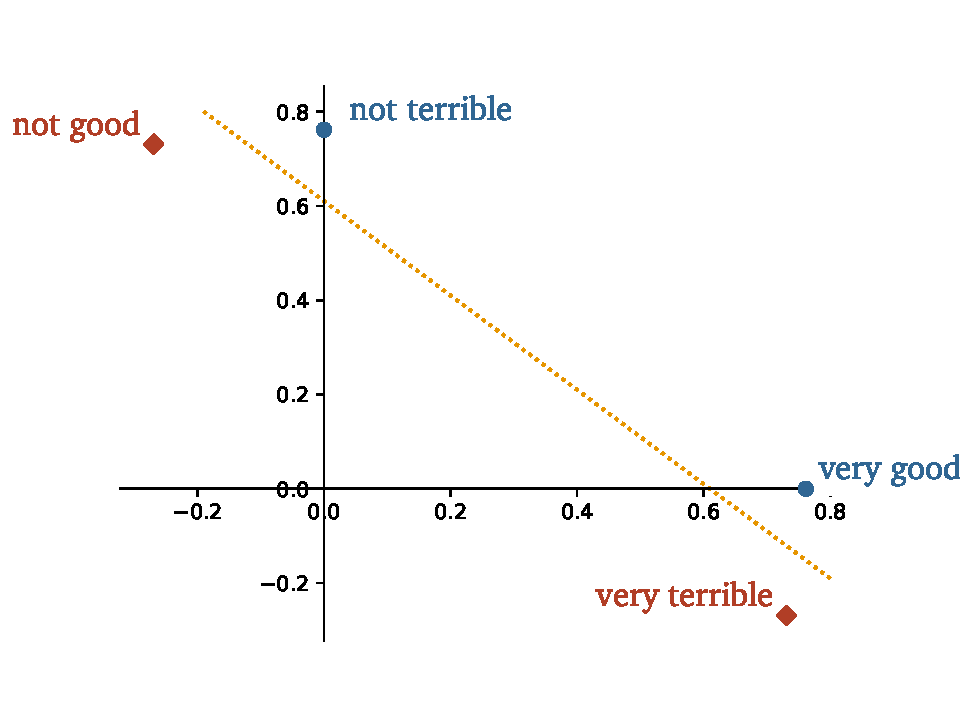
\includegraphics[width=0.9\linewidth]{./images/attention/notvery.pdf}
\vspace{-2em}
\end{figure} \qed
\end{proof}

I found this solution through a bit of trial and error. There isn't much intuition I can discover in the way the self attention solves the problem. One thing worth noting is that it doesn't solve the problem by the properties of multiplication. This is the more obvious way to solve if/then-style problems like this one and the XOR problem: you represent the \texttt{not} by a negative number and apply it to the sentiment of the \texttt{good} ($+1$) and the \texttt{terrible} ($-1$) by multiplication. This, the self attention cannot do, or at least not directly. There is a multiplication in the computation of the weights, but ultimately, the vectors representing the different words are just added together.

This approach just about works for the not/very problem, but it has its limits. Theorem \ldots from the last chapter shows that a self-attention by itself cannot solve the sequential XOR problem: self-attention produces a weighted sum, with the weights determined by the input, so the theorem applies.

In fact, the output of the self-attention for the XOR problem follows a fixed pattern, regardless of how we set the embedding vectors. We start with the outputs for ``true true'' and ``false false''. However we set the weights we get a weighted sum of two terms where both terms are either $\oc{\mbv}_t$ or $\oc{\mbv}_f$, so the output is \emph{also} $\oc{\mbv}_t$ or $\oc{\mbv}_f$, resprectively. 

For the two inputs \texttt{true false} and \texttt{false true}, the result is always of the form
\[
\oc{w}_{a}\oc{\mbv}_t + \oc{w}_b \oc{\mbv}_f
\]
where the two weights are positive and sum to one. That is, these outputs are a \emph{convex combination} on the vectors $\oc{\mbv}_t$ or $\oc{\mbv}_f$, so they must lie on the line segment between these two points. 

\index{Convex combination}

For example, if we set 
\[
\oc{\mbv}_t = \begin{pmatrix}1\\0\end{pmatrix} \;\;\; \oc{\mbv}_f = \begin{pmatrix}0\\1\end{pmatrix}
\]

we get the following result for the first output vector.

\begin{figure}[H]
\centering
	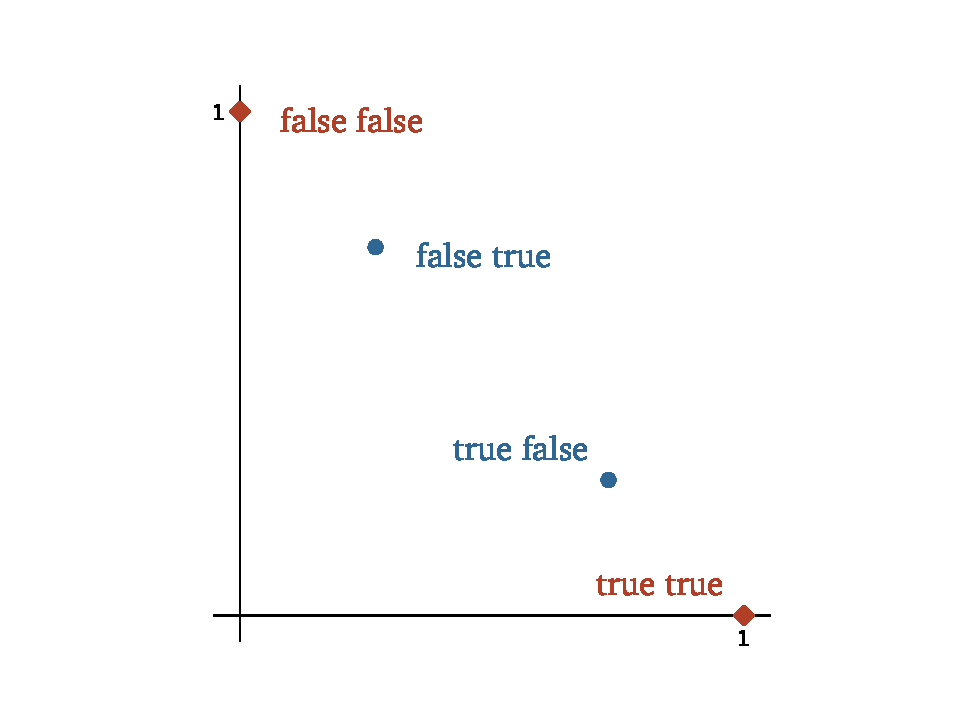
\includegraphics[width=0.9\linewidth]{./images/attention/xor.pdf}
\end{figure}

The two classes are not linearly separable, but they can be separated by a simple \emph{nonlinear }decision boundary. We could for instance, draw a circle around the two positive points.

This is the key to what self-attention does for us: it doesn't solve any complex problem, but it mixes together the different vectors in the input in a coordinated way. Compare this to what we would get if we selected the first vector before the self attention: we would only get the  representation of the first word, regardless of the other words in the input sequence. When we select the first output vector \emph{after} the self-attention, all four possible inputs lead to different values.

The way to solve the XOR problem with a self-attention is to pair it up with a mechanism that can take the situation above, and transform it so that the vectors become linearly separable. In the appendix, we show that a single two-layer feedforward network with ReLU activations can draw the required decision boundary, so long as its hidden layer is bigger than its input layer.

% pointwise

This means that we can pass each output vector of the self attention through one such feedforward network, and end up with perfectly linearly separable classes. 

This is is a very powerful idea: we use self-attention, with its limited power to propagate information between the words in the input sequence, adding information to each vector about what is happening elsewhere in the sentence. Then, we pass each vector, in isolation, through the same feedforward network. The feedforward network doesn't see what's happening elsewhere in the sentence, but the self-attention has already placed that information in every individual vector. 

When we start building transformers, we will see that the combination of self-attention and feed-forward layers is a key aspect of the architecture.

\subsection{Decoupling linearity and nonlinearity}

Another aspect of the self-attention that is worth showing in detail is the way it decouples its linear and nonlinear computations. At heart, the self-attention is nothing more than a matrix multiplication:
\[
\mbY = \mbX \oc{\mbW} \p 
\]

If we ignore the fact that the weights, are derived, and only look at the gradients for the input $\bc{\mbX}$, we get perfectly non-vanishing gradients from $\mbY^\nabla$ to $\bc{\mbX}^\nabla$.

% Go into vanishing gradients and linear operations in the appendix

Of course, this isn't the only way in which the values of $\bc{\mbX}$ influence the value of $\mbY$. There is a second path of computation from $\bc{\mbX}$ to $\oc{\mbW}$. We can draw this in a computation graph as follows.

-- Diagram

By the multivariate chain rule we can compute the complete gradient by working out the gradients for both paths and summing them together. This means that our complete gradient is the sum of a linear, non-vanishing gradient, and a non-linear vanishing gradient.

This is most likely a big reason for why self attention works so well, when stacked deeply. Imagine that we build a model, consisting of a single embedding layer, followed by a stack of  16 simple self-attentions. If we ignore the non-linear aspect of the self-attention, what we are looking at, is a stack of 16 matrix multiplications without non-linearities. 

We can backpropagate a gradient through such a computation perfectly, so that the embeddings at the bottom of our model can readily be trained with a strong gradient. In this perspective, the embeddings are trained to do their job well, given that they will be passed through 16, more or less random matrix multiplications. We are, in effect, training the embeddings under the assumption that these matrices will remain constant. They won't, but since they will change slowly, this is still a reasonable assumption. 

On a second, slower level, there is a gradient that adapts embedding vectors to optimize the matrices themselves. This gradient is backpropagated through a softmax operation, so we can expect it to be smaller and to operate much more slowly: especially for the earlier layers, the gradient will have decayed a lot.

\subsubsection{The complete gradient}

Using an automatic differentiaton system means never having to work out your gradients. If you can implement the forward, you can let Pytorch, Tensorflow or JAX worry about the backward. Still, sometimes it's useful to work out the backward pass yourself. This can be because you suffer from numerical instabilities, in which case you can take the naive implementation of the backward and rework it into something more stable, or just because you want to analyse how the gradients flow, and what it means for your model, much like we did in the last section.

We'll go the distance in this section, and provide the full backward for attention and self-attention. If you have an automatic differentiation system, you won't get much benefit from implementing this manually, and it won't tell us much more that the previous section, but it's worth having here for completeness.

We'll start with general attention. Let $\rc{\mbV}$, $\gc{\mbK}$ and $\bc{\mbQ}$ be the matrices containing the \rc{value}, \gc{key} and \bc{query} vectors as their columns. The attention operation proceeds in three steps, but we'll break up the softmax step into three separate steps: exponentiation summing/expanding the columns and normalizing. This gives us the following five steps for the full attention

\begin{align*}
\oc{\mbW}_r  &= \gc{\mbK}^T\bc{\mbQ} & \text{compute the raw weights}\\	
\oc{\mbW}_e &= \exp \, \oc{\mbW}_r & \text{exponentiate the raw weights}\\
\oc{\mbW}_s &=  \one\one^T \oc{\mbW}_e & \text{sum and expand the columns}\\	
\oc{\mbW} &= \oc{\mbW}_e \soslash \oc{\mbW}_s & \text{normalize}\\	
\mbY &= \rc{\mbV} \oc{\mbW} &\text{compute weighted means} \p 
\end{align*}

Which, in diagram form looks as follows.

-- Diagram

These are all steps for which the gradients are given in Appendix~\ref{ch:deep-learning}.

 matrix multiplication (Theorem~\ref{thm:matmult}), element-wise exponentiation (Theorem~\ref{thm:elem-wise}, Corollaries 1 and 4) and column normalization (Theorem~\ref{thm:colnorm}).

Applying these results, we get 

\begin{align*}
\rc{\mbV}^\nabla &= \mbY^\nabla \oc{\mbW}^T & \text{Theorem~\ref{thm:matmult}}\\
\oc{\mbW}^\nabla &= \rc{\mbV}^T \mbY^\nabla & \text{Theorem~\ref{thm:matmult}}\\
\oc{\mbW}_s^\nabla &= \oc{\mbW}^\nabla \sotimes \oc{\mbW}_e \soslash - {\oc{\mbW}_s}^{\circ 2} & \text{Theorem~\ref{thm:elem-wise}, Cor. 4, Theorem~\ref{thm:matmult}} \\
\oc{\mbW}_e^\nabla &= \oc{\mbW}^\nabla \soslash {\oc{\mbW}_s}^{\circ 1} + \one\one^T \oc{\mbW}_s^\nabla & \text{Theorem~\ref{thm:elem-wise}, Cor. 4}\\
\oc{\mbW}_r^\nabla &= \oc{\mbW}_e^\nabla \sotimes \exp \oc{\mbW}_r & \text{Theorem~\ref{thm:elem-wise}, Cor. 1}\\
\gc{\mbK}^\nabla &= \bc{\mbQ} \oc{\mbW}_r^{\nabla T} & \text{Theorem~\ref{thm:matmult}}\\
\bc{\mbQ}^\nabla &= \gc{\mbK}\oc{\mbW}_r^{\nabla} & \text{Theorem~\ref{thm:matmult}.}\hspace{-0.32em}
\end{align*}

\begin{aside}
Note that $\oc{\mbW}_e$ is used in the computation of two variables upstream ($\oc{\mbW}_s$ and $\oc{\mbW}$), so its gradient is a function of two upstream gradients.
\end{aside}

Expanding these variables won't allow us to simplify them much, so this is probably the way you would want to implement it (which is what an AD does for you automatically). However, we can focus on the gradients for the inputs and expand them a little, to emphasize the point in the previous section:

\begin{align*}
\rc{\mbV}^\nabla &= \mbY^\nabla\oc{\mbW}^T	\\
\gc{\mbK}^\nabla &= \bc{\mbQ}(\oc{\mbW}_e^\nabla \sotimes \exp \oc{\mbW}_r) 	\\
\bc{\mbQ}^\nabla &= \gc{\mbK}(\oc{\mbW}_e^\nabla \sotimes \exp \oc{\mbW}_r)^T \p \\
\end{align*}

This shows that in the computation of $\gc{\mbK}^\nabla$ and $\bc{\mbQ}^\nabla$, we element-wise multiply our upstream gradients $\oc{\mbW}_e^\nabla$ by \emph{the exponentiated} raw weights $\exp \oc{\mbW}_r$. The \rc{value} gradients $\rc{\mbV}^\nabla$ by constrast, are computed by a simple matrix multiplication by a given matrix $\oc{\mbW}$.

\subsection{Permutation equivariance}
\index{Permutation equivariance}

A second property of self-attention that is important to understand goes by the fancy name of \emph{permutation equivariance}. Put simply, it means that if we shuffle the words in the input sequence, the words in the output sequence will be shuffled in the same way. 

Say we run a sequence like $\oc{\mbv}_\text{the}, \oc{\mbv}_\text{cat}, \oc{\mbv}_\text{walks}$ through a self attention, and observe some output vector $\mby_\text{walks}$ in the last position. If we then run the sequence $\oc{\mbv}_\text{walks}, \oc{\mbv}_\text{the}, \oc{\mbv}_\text{cat}$ though the self attention, we will get the same output vector $\mby_\text{walks}$, but in the \emph{first position}.

\begin{aside}
Note that the embedding layer is also permutation equivariant. If we shuffle the words in our input sentence, we get the same sequence of embedding vectors, but shuffled in the same way.	
\end{aside}


This is especially relevant for the sentiment classification model we are using currently, because the gobal pooling layer (a mean pool) that we use is \emph{permutation \textbf{in}variant}: any permutation of a given input will always lead to the same output. This is because the mean is essentially a sum, with a constant multiplier. For sums, it doesn't matter in what order you sum the terms, the result is always the same.

The result of chaining together equivariant operations like the embedding layer and the self-attention, with an invariant operation like the global mean pool, is an \emph{invariant model}. If we take two sentences like
\begin{itemize}
\item This is not a filthy burger joint, it's a real restaurant.
\item This is not a real restaurant, it's a filthy burger joint. 
\end{itemize}
We see that the model must assign them the same label. The outputs of the embedding layer and self-attention are the same sequence of vectors, just in a different order, and the output of the global pool is the same for any two sequences that are permutations of one another.

Since these two sentences have opposite sentiments, the model must misclassify one of them. More generally, it shows that we still have a bag-of-words model. In a sense, the model cannot ``see'' the order of the words in the sentence. 

There are some simple ways around this, which we will introduce in the next chapter. For now, the main takeaway is that the self-attention by itself is more of a \emph{set model} than a \emph{sequence model}. We may feed the model a sequence, but all it really represents is the set of words that occur in the sequence. It ignores which order we feed them in.

\begin{aside}
Strictly speaking, it represents the multiset, since it can represent the fact that a word occurs multiple times. 	
\end{aside}

We are appealing to intuition a little bit in saying that the properties of permutation equivarance and invariance translate to a model that treats its input as a set. However, this connection can be made more precise. There is a close, and mathematically precise, connection between the types of transformations you can apply to an object, without its representation changing, and the type of object you are dealing with. We will dig a little deeper into this connection in Chapter~\ref{}.

\subsubsection{Proving permutation equivariance}
\index{Permutation equivariance!Proof}

Since permutation equivariance is such a key property for self-attention, it's worth taking the time to prove it properly. We'll start by defining it more precisely and generally.

First, we will refer to a permutation as $\pi$, and to the result of permuting some sequence $S = \mbs_1, \ldots, \mbs_n$ as $\pi S$. That is,  $\pi S$ represents the shuffled sequence.

We can now say that a function $f$ from sequences to sequences is equivariant to permutation $\pi$ if $f (\pi S) = \pi f(S)$, for all $S$. That is, we get the same result whether we shuffle first and then apply the function $f$ or apply $f$ first and then shuffle. Any function that is equivariant to all permutations is permutation equivariant.

If a function has multiple inputs or outputs, like attention does, then we apply the same single permutation to all inputs and to all outputs.

This definition is often expressed in a commutation diagram:

-- Diagram

\begin{aside}
The name comes from the fact that two operators that can be applied in either order, with the same result, are said to \emph{commute}.	
\end{aside}

This is equivalent to how we defined permutation equivariance earlier: if we shuffle the input sequence ($\pi$), the result is the same as without the shuffle ($f(S)$) except shuffled also ($\pi f(S)$).

Before we look at the self-attention, let's look at the simpler example of the embedding layer. This is an example of a layer that doesn't propagate information across the sequence dimension. That is, for output $i$, it will only look at \emph{input} $i$, ignoring the values in the rest of the sequence. We call these \emph{pointwise layers}. 
\index{Pointwise layer|textbf}

\begin{theorem}[Pointwise layers]\label{thm:pointwise-permeq}
	Any point-wise sequence-to-sequence layer $f$ is permutation equivariant.
\end{theorem}
\begin{proof}
Let $\pi$ and $S$ be any permutation and sequence. Let $f^.$ be the function that $f$ applies to each element of its input individually. Let $i$ be any index that is mapped to $j$ under the permutation.
\[
(\pi f(\mbS))_j = f(\mbS)_i = f^.(\mbs_i) = f^.((\pi S)_j) = f(\pi S)_j \p \hfill
\] \qed
\end{proof}

As a corollary, our embedding layer is permutation equivariant, as is the feed-forward layer we introduced to solve the XOR problem.

Next, let's look at attention.

\begin{theorem}[Attention is permutation equivariant]\label{thm:attn-permeq}
\end{theorem}
\begin{proof}
Let $\rc{\mbV}, \gc{\mbK}, \bc{\mbQ}$ be any three input sequences of vectors represented as a matrices in the default way. Let $\mbP$ be any permutation, represented as a permutation matrix, so that $\mbP\mbX$ is the permutation of vector sequence $\mbX$ by $\mbP$.

\begin{align*}
 f(\mbP\rc{\mbV}, \mbP\gc{\mbK}, \mbP\bc{\mbQ}) &=  \mbP\rc{\mbV}\, \text{softmax}\left(\kc{k^{-1}} (\mbP\gc{\mbK})^T\mbP\bc{\mbQ}\right) \\
  &=  \mbP\rc{\mbV}\, \text{softmax}\left(\kc{k^{-1}} \gc{\mbK}^T\mbP^T\mbP\bc{\mbX}\right)\\
  &=  \mbP\;\rc{\mbV}\, \text{softmax}\left(\kc{k^{-1}} \gc{\mbK}^T\bc{\mbQ}\right)  \;\;\;\mbP^T\mbP = \mbI \\
    &=  \mbP\,f(\rc{\mbV}, \gc{\mbK}, \bc{\mbQ}) \p 
\end{align*}\qed
\end{proof}

If we set $\bc{\mbX} = \rc{\mbV} = \gc{\mbK} = \bc{\mbQ}$, then it follows as a corollary that simple self-attention is also permutation equivariant.



\section{Full-fledged self-attention}

What we have described  so far is \emph{almost} self-attention as it's used in every multi-million dollar model today. There are just two more features to add: projections, and multi-head self-attention.

\subsection{Key, query and value projections}

First, note two properties of the self-attention we have defined so far.

\begin{description}
\item[It doesn't have any parameters] The behavior of the simple self-attention is driven entirely by what's in the input vectors. This works pretty well, since whatever is upstream of the self-attention is usually learned by us. Still, a little more control doesn't hurt, especially if we would like to apply multiple self-attentions in parallel, and have them behave differently.
\item[The weight from input $i$ to output $i$ is usually the highest] It's possible to come up with examples where this isn't true, but by-and-large, the dot product of a vector is bigger with itself than it is with other vectors. The vectors that we commonly encounter will usually all point in different directions, and be roughly the same length. This means that the output at position $i$ will mostly be the input at $i$, but with a little bit of its neighbors mixed in. This is not a bad mechanism, especially if the inputs are embedding vectors that already work pretty well by themselves. Still, it's not necessarily what we always want to happen. Especially, again, if we want multiple self-attentions to operate in parallel, doing different things.
\item[Simple self-attention is symmetric] That is, the matrix $\oc{\mbW}$ of attention weights is symmetric. This means that in a sentence like ``This restaurant was not terrible.'', we must always put as much of the representation of \texttt{not} into \texttt{terrible} as the other way around. Again, this may not always be a bad thing, but it would be nice to be able to control it. 
\end{description}

All three problems can be solved by a simple trick: we add a single linear layer to each input of the self attention. So, instead of saying $\rc{\mbV} = \gc{\mbK} = \bc{\mbQ} = \mbX$, we say 
\begin{align*}
\rc{\mbV} &= \mbW_\rc{v}{\mbX} + \mbb_\rc{v} \\	
\gc{\mbK} &= \mbW_\gc{k}{\mbX} + \mbb_\gc{k} \\	
\bc{\mbQ} &= \mbW_\bc{q}{\mbX} + \mbb_\bc{q}
\end{align*}

Where the \emph{weights} $\mbW$ are $k \times k$ parameter matrices, and the \emph{biases} $\mbb$ are parameter vectors of $k$ dimensions.

\begin{aside}
There is a slight abuse of notation here, in that the bias vector is added to each column of the matrix it's summed with. Many recent models omit the bias vectors, so think of them as optional features. 
\end{aside}

With this, we have a \emph{parametrized} self-attention. The main driver of the behavior is still the content of the input vectors itself, but there is some control in how the keys are matched to the queries and in what values are returned. 

As we noted above, this is especially useful if we want to apply multiple self-attentions in parallel.

\subsection{Multi-head self attention}

The first obvious question is why would we want to? Why run, say, four self attention operations in parallel, when you can also run them in sequence, using the output of one as the input of the next?

One answer is that parallel processing is usually more efficient than sequential processing. It also has some downsides. For example in a parallel configuration, what the second self-attention does cannot depend on what the first is doing. That's pretty much the definition of parallel processing. 

So, the real question is perhaps, do we expect this to be valuable? Considering the sort of thing we expect the self-attention to do, can we expect it to be useful to do two or more of such things in parallel?

\begin{aside}We have to be a bit careful here. Quite often such architectural features are introduced with some idea about what the model may need to do, and then shown to improve performance. However, when we then investigate, we may find that the trained model, even though it makes use of the feature, is using it in a completely different way from our initial intuition.
\end{aside}

Our conceptual model of self-attention is that it mixes word embeddings. At the start of our model, we have only embeddings for each word in isolation. The representation $\oc{\mbv}_\texttt{terrible}$ is necessarily the same for every occurrence of the word \texttt{terrible}, regardless of context. The self-attention looks at the surrounding embedding vectors and mixes some relevant aspects into the resulting representation of the word \texttt{terrible}. The result is that our representation of the word now conveys not just what the word means in general, but what it means \emph{in this particular context}.

In natural language, there are certainly many different relations between words that can be extracted in parallel. Here is an example:


This movie's lead actor was not too terrible.	

% Add pointers

The word \texttt{terrible} expresses a sentiment. This sentiment is tempered by \texttt{too} and then inverted by \texttt{not}. To understand the subtle sentiment expressed in the sentence, we need to process how these three words interact. The relation between \texttt{terrible}, \texttt{movie} and \texttt{actor} is different. The latter two words don't affect the sentiment expressed, but \emph{about whom} the sentiment is expressed. We'd like this information to be aggregated into our representation of \texttt{terrible}, together with the sentiment.

These two aspects are relatively orthogonal. What exactly the sentiment is, and who it is about can be worked out independently of each other, from very different parts of the sentence. This suggests we could get a benefit from running different self-attention operations in parallel. We'll develop a feature that allows us to experiment with this. We'll then simply tune the number of parallel operations, and pick the number that leads to the best performance.

 Once we've discussed large trained models, we'll return to this question. We'll try some techniques for inspecting the internals of the model, to see whether our intuitions about parallel processing were justified.

We call the different parallel self-attentions \emph{heads}. A collection of self-attention operations applied in parallel is called a \emph{multi-head self-attention}.

\subsubsection{Naive multi-head self-attention}

Say we've decided to build a model consisting of an embedding layer, and 6 self-attention blocks, each with their own query, key and value projections. We could first of all, put all 6 self-attentions after each other, using the output of one as the input to the next. Call this the \emph{fully sequential} model.

We could also run all of them in parallel. We compute the embedding vectors, feed these to each of the 6 attentions, which are then computed independently of what is happening in the others. At the end, we get 6 sequences of output vectors, which we would have to combine somehow into a single sequence. For the sake of simplicity we can just average them: that is, the first output vector of the comvined multi-head self attention is the average of the first output vectors of all 6 self attentions. Call this the \emph{fully parallel model}. 

If we ignore the training time, the fully sequential model would probably work best. It can do something that the fully parallel model can't: let the behavior of one self-attention operation depend on the output of another. However, the full parallel model can be parallelized much better, and so will likely run faster, seeing more data per second, so on  hardware suited to parallelization, like a GPU, the parallel model may yet win out. 

This is especially promising is there are aspects of the problem that are naturally parallel. For example, as noted above, working out what noun the word \texttt{terrible} is a property of and working out whether its negative sentiment is negated by the word \texttt{not}.

In practice, we can't usually perfectly predict how much inherent parallelism our task allows, so we need to try and see. In between the full parallel and the fully sequential models, there are many different options. There are the most regular:

-- diagram seq, 2x3, 3x2, parallel

Which option works best for us depends on the nature of the task and the properties of the data. We call the parallel application of 2, 3 or 6 self-attentions a multi-head self-attention.

In this set-up---the \emph{naive} self-attention---we pay more or less the same for each attention block. The parallel ones can be computed more efficiently, but each block by itself still takes the same amount of time to compute. 

It turns out, however, that with a little cleverness, we can have our cake and eat it too. We can compute a multi-head self-attention using roughly the same amount of time and memory it takes to compute a single regular self-attention. The way we do this is by first projecting down to a lower-dimensional space. 

\subsubsection{Efficient multi-head self-attention}

Assume that we have a fully sequential model, and we want to replace each self-attention, on vectors of dimension $k$, by 4 parallel self-attention s. We will try to do this in a way that uses about the same number of parameters, the same amount of computation and the same amount of memory that the single self attention does.

The basic idea is simple. It consists of the following steps:
\begin{enumerate}
	\item Project the input vectors down to a 4 separate vectors sequences of dimension $k/4$ (we assume that $k$ is divisible by $4$).
	\item Feed each of these sequences of smaller vectors into its own self-attention, with its own query, key and value projections. 
	\item Take the 4 output sequences and concatenate them into a sequence of the vectors dimension $k$.
	\item (optional) Apply a linear $k\times k$ transformation $\mbW_0$ to mix up the embeddings. 
\end{enumerate}

To show that this is not much more complex than a regular single self-attention, we can first investigate the first two steps. Note that these are both linear operations, and that the output of one is fed directly into the other. That suggests that we can combine them into a single linear operation, since two linear operations composed just makes another linear operation. 

In practice, this looks as follows. The operations described above projects down to $k/4$ by a  $k \times k/4$ matrix $\mbD$ and then multiplies by a 
$k/4 \times k/4$ matrix $\bc{\mbQ}x$ to the \bc{queries}. We get the same result if we multiply $\mbD\bc{\mbQ}$ which gives us a $k/4 \times k$ matrix. Instead of using $\mbD$ and $\bc{\mbQ}$ as parameters of our model, we just use this $k/4 \times k$ matrix. 

-- diagram

The following diagram shows that if we do this for all queries, keys and values of the four heads, we end up with the equivalent of three $k \times k$ matrices. Exactly the same number of parameters we would use if we had just a single self-attention. 

\begin{aside}
The same holds for the biases. We get 3 bias vectors of dimension $k$ each, or $3 \cdot 4$ bias vectors of dimension $k/4$ each.
\end{aside}
 
With one matrix operation, we've projected the the input vectors down to $3 \cdot 4$ vector sequences of dimension $k/4$ which can serve as the queries, keys and values of $4$ separate self-attention operations. 

After these operations are done, we concatenate their outputs, so that we once again have a sequence of vectors of dimension $k$. Optionally, we apply one final multiplication by a $k \times k$ parameter matrix $\mbW_0$, to mix up the dimensions. Here is the whole operation in a single diagram.

-- diagram

\begin{aside}
The transformation by $\oc{\mbW_0}$ is a bit of an odd duck. Without it, as shown below, the computation of the regular self attention costs almost exactly the same as a multi-head self-attention. However, that is before we include the multiplication by $\oc{\mbW_0}$. Moreover, as we will see in the next chapter, almost all transformers add some feedforward layers after the self attention, so that the dimensions are mixed up anyway. In short, it would be much neater to build multi-head self-attention without $\oc{\mbW_0}$, but the canonical version includes it.
\end{aside}

\emph{Implementation}

The trick to implementing multi-head self-attention efficiently is to treat the different heads as a new dimension. Note that, since we have a batched implementation, we are \emph{already} computing multiple self-attentions in parallel. All we really need to do is add another dimension for the heads, make sure that that dimension is treated as a batch dimension. 

First, let's write a general attention operation.

\begin{alltt}
\textbf{function} attention(\bc{queries}, \gc{keys}, \rc{values}):

\tab \oc{raw_weights} ← \gc{keys} @ \bc{queries}.T
\tab \oc{raw_weights} ← \oc{raw_weights} / sqrt(k)

\tab \oc{weights} ← softmax(\oc{raw_weights}, dim=-2)

\tab \textbf{return} \rc{values} @ \oc{weights}
\end{alltt}

Here, the \texttt{@} operator represents matrix multiplication. We assume that this operates on the last two dimensions, and treats the rest as \gc{batch dimensions}. For example, if \texttt{x} is a 4-tensor with dimensions $\gc{3}, \gc{7}, 5, \rc{9}$ and \texttt{y} is a tensor with dimensions $\gc{3}, \gc{7}, \rc{9}, 10$ then \texttt{x @ y} performs a multiplication of a $5 \times \rc{9}$ matrix with a $\rc{9} \times 10$ matrix for every index in the first $\gc{3}, \gc{7}$ dimensions. The result is a 4-tensor with dimensions $\gc{3}, \gc{7}, 5, 10$.

-- diagram (batches as matrix, single index as matrix)

Note that the attention expects the last two dimensions to be time and embedding respectively. 

\begin{aside}
Most tensor computation libraries, like Numpy and Pytorch, have such a matrix multiplication function, but be sure to read the documentation carefully. Often there are different functions with and without batching. 
\end{aside}

With this function in place, all we need to do is extract the keys, queries and values for the different heads into an extra dimension. 

First, we set up four linear layers with $k$ inputs and $k$ outputs. 

\begin{alltt}
\bc{toqueries} ← Linear(k, k)
\gc{tokeys}    ← Linear(k  k)
\rc{tovalues}  ← Linear(k, k)

unifyheads ← nn.Linear(k, k)	
\end{alltt}

The first three extract the \bc{queries}, \gc{keys} and \rc{values} for all heads. The last is the concatenation function $\mbW_0$.

\begin{aside}
Most commonly, the first three do not include biases, and the last does. We will leave this detail out of the implementation for the sake of simplicity.	If we wanted to be super-efficient we could replace the first three by one linear layer with $k$ inputs and $3k$ outputs, but we are making a small tradeoff for readability here.
\end{aside}


Next, we assume we are given our input sequence as a 3-tensor \texttt{x}, with dimensions, in order: batch, time, embedding. That is, \texttt{x[\rc{3}, \bc{5}, :]} is the embedding vector for the \bc{sixth} token in the input sequence of the \rc{fourth} instance in the batch (note that we are assuming 0-indexing). 

We assume that \texttt{h} is the number of heads.

\begin{alltt}
b, t, k ← x.size()

\textbf{assert} k \% h = 0

s = k // h \gc{\# embedding dim per head }

\bc{queries} ← \bc{toqueries}(x)
\gc{keys}    ← \gc{tokeys}(x)
\rc{values}  ← \rc{tovalues}(x)

\end{alltt}

At this point the queries, keys and values are tensors of size \texttt{b, t, k}. That is, the last dimension contains all vectors for all heads, concatenates into a single vector of length \texttt{k}. To break this up, we simply keep the same data in memory, but \emph{view} is as a tensor of different dimensionaliuty.

\begin{alltt}
\bc{queries} ← \bc{queries}.view(b, t, h, s)
\gc{keys}    ← \gc{keys}.view(b, t, h, s)
\rc{values}  ← \rc{values}.view(b, t, h, s)	
\end{alltt}

To see how this works, note that all tensors are stored in memory as a single list of numbers. A matrix of size $2 \times 3$ is stored in compute memory simply as a list like

\[
1,2,3,4,5,6
\]

We turn this into a matrix, by combining it with the information that the matrix has two rows and three columns. This tells us that the first three numbers in the list (1,2,3) are the first row and the rest form the second row (4, 5, 6). The same data with a different size, say $3\times 2$ forms a different matrix:
\[
\begin{pmatrix}
	1& 2 \\
	3&4 \\
	5&6 \\
\end{pmatrix}
\]

We can even change the dimensions. This data can also be viewed as a single vector of dimension 6.

This is what's happening above. We have 3-tensors of size \texttt{\gc{b}, \gc{t}, k}. In this operation, the dimensions \texttt{\gc{b}, \gc{t}} stay the same. In other words, we treat them as \emph{batch dimensions}: we simply apply the same operation individually to each index in the first two dimension. So, ignoring these batch dimensions, what do we have? We start with a single vector of length \texttt{k} and we \emph{view} it as a matrix of size \texttt{h,s}.

-- diagram.

In this matrix, each row represents the query, key or value for a particular head.

\begin{aside}
The \texttt{view} operation is sometimes called \texttt{reshape}. See the Appendix for more details.
\end{aside}

Next, we need to feed these to the attention operation. This requires us to shuffle the dimensions, since the attention expects the last two dimension to be time \texttt{t} and embedding \texttt{s}. 

\begin{alltt}
\bc{queries} ← \bc{queries}.transpose(1,2)
\gc{keys}    ← \gc{keys}.transpose(1,2)
\rc{values}  ← \rc{values}.transpose(1,2)
\end{alltt}

\begin{aside}
Depending on the details of your platform, you may need to make these tensors contiguous first. That is, create a copy for which the data in memory is in the right order.
\end{aside}

We can now pass these tensors to our attention operation.

\begin{alltt}
result ← attention(\bc{queries}, \gc{keys}, \rc{values})
\textbf{assert} result.size() = b, h, t, s
\end{alltt}

This computes the attention for all heads in parallel. Now all we need to do is concatenate the output. To do this, we first transpose the dimensions again so that the head and embedding dimensions are next to each other, and then reverse the view operation to get back from an $h \times s$ matrix to a $k$ vector.

\begin{alltt}
result ← result.transpose(1,2).view(b, t, k)
result ← unifyheads(result)
\end{alltt}


\section{Revisiting classification}

With our multi-headed self-attention operation fully fleshed out, we can return to our classification task, and see if adding attention to our bag-of-words model has any effect.

To keep things as simple as possible, we will just insert one self-attention operation between the embedding layer and the global pooling. 

-- diagram

% Run this
% Do some inspection?

\section{Masking}

\subsection{Variants of attention}

\subsubsection{Linear attention}

\subsubsection{Sparse attention}

\subsubsection{Other tricks}

\subsection{Historical overview}

\chapter{The transformer}

\section{The transformer \emph{block}}

\subsection{Normalization}
\subsection{Dropout}
\subsection{Residual connections}

% Discuss vanishing gradient principle

\subsection{Feedforward connections}

\chapter{Pre-training}

\section{Autoregressive pre-training}

\chapter{Scaling up}

% Historical overview

\section{Masked language modeling}

\section{Autoregressive models}

\subsection{GPT-2 (2019)}

\section{Multi-process and multi-node training}

\subsection{Hogwild}

\subsection{Data-parallel}

\subsection{FSDP}

\subsection{Other options}

\subsubsection{Distillation}

\chapter{In-context learning}

\chapter{Other architectures}

\section{The perceiver}

\section{Encoder/decoder models}

\section{Recurrent models}


\chapter{Images and other grids}

\section{Architectures}

\section{Pre-training and finetuning}

\chapter{Audio and other high frequency sequences}

% Audio, EEG, etc.

\chapter{Graphs and other relational data}

\chapter{Equivariance: modeling your problem}

\appendix

\chapter{Mathematical preliminaries}
\label{ch:preliminaries}

\section{Notation and basic concepts}

\section{Calculus}

Follow the lecture, only derivatives and gradients.

\subsection{The chain rule(s)}
\subsubsection{The multivariate chain rule}

\section{Linear Algebra}

\begin{itemize}
\item All vectors are column vectors
\item Doooooot products
\item Inner, outer product definition of matrix multiplication.	
\item Using $\one$ to sum, expand, etc.
\end{itemize}

\chapter{Machine learning}

\begin{itemize}
	\item Overfitting
	\item XOR problem, circle problem
	\item Linear models, gradient descent.
\end{itemize}

\section{Abstract tasks}

\subsection{Generalization}
\subsection{Is Machine Learning a probabilistic discipline?}
\section{Feature space and model space}
\section{Optimization and gradient descent}
\subsection{Momentum and Adam}

\chapter{Neural networks and deep Learning}

\begin{itemize}
    \item using NNs to solve the XOR and circle problem
    \item Universal approximation?
    \item Large hidden layers are required for closed shapes.
    \item Vanishing gradients
	\item Vectorization
	\item Hyperparameter optimization.
	\item Batching, throughput
\end{itemize}

\section{Neural networks}

\subsection{Nonlinear problems}

\subsection{What's ``neural'' about it? }

\section{Working out the gradient}

\subsection{Local and global derivatives}

\subsection{Scalar backpropagation}

\subsection{Tensor backpropagation}

\subsubsection{Should we be using matrix or vector calculus?}

\subsubsection{Tensor backpropagation from scalar derivatives}

\subsection{Automatic differentiation}

\subsubsection{No more pen and paper}

\subsubsection{Some example backwards}

We can help ourselves think about gradient propagation, by building up a small vocabulary of worked out backwards functions for common operations. Working these out, or at least following the workings out should help to internalize the recipe. 

These are the backwards functions that we will use throughout the book.

To avoid double or triple supercripts, we will sometimes write them on the same level. For example ${\bc{\mbX}^\nabla}^T = \bc{\mbX}^{\nabla T}$.

\begin{theorem}[Matrix multiplication] \label{thm:matmult}
If $\bc{\mbC} = \rc{\mbA}\gc{\mbB}$ then $\rc{\mbA}^\nabla = \bc{\mbC}^{\nabla}\gc{\mbB}^T$ and $\gc{\mbB}^\nabla = \rc{\mbA}^T\bc{\mbC}^{\nabla}$.
\end{theorem}
\begin{proof}
\begin{align*}
\rc{A}_{ij}^\nabla &= \frac{\kp l}{\kp \rc{A}_{ij}} = \sum_{kl} \frac{\kp l }{\kp \bc{C}_{kl}} \frac{\kp \bc{C}_{kl}}{\kp \rc{A}_{ij}} = \sum_{kl} \bc{C}_{kl}^\nabla \frac{\kp [\rc{\mbA}\gc{\mbB}]_{kl}}{\kp \rc{A}_{ij}} \\	
&= \sum_{kl} \bc{C}_{kl}^\nabla \frac{\kp \sum_\kc{m} \rc{A}_{k\kc{m}}\gc{B}_{\kc{m}l}}{\kp \rc{A}_{ij}} = \sum_{kl\kc{m}} \bc{C}_{kl}^\nabla \frac{\kp \rc{A}_{k\kc{m}}\gc{B}_{\kc{m}l}}{\kp \rc{A}_{ij}} \\
&=  \sum_{l} \bc{C}_{il}^\nabla \frac{\kp \rc{A}_{ij}\gc{B}_{jl}}{\kp \rc{A}_{ij}} = \sum_{l} \bc{C}_{il}^\nabla \gc{B}_{jl}  = \sum_{l} \bc{C}_{il}^\nabla \gc{B}^T_{lj}
\end{align*}
Note that the last part can be interpreted as a dot product. If element $ij$ of $\rc{\mbA}^\nabla$ can be written as a dot product between the $i$-th row of \bc{one matrix} and the $j$-th column of \gc{another}, then, by the definition of matrix multiplication, $\rc{\mbA}^\nabla$ is the product of these two matrices:
\[
\rc{\mbA}^\nabla = \bc{\mbC}^\nabla \gc{\mbB}^T \p 
\]
Similarly, for $\gc{\mbB}^\nabla$:

\begin{align*}
\gc{B}_{ij}^{\nabla} &= \sum_{kl} \bc{C}^\nabla_{kl} \frac{\kp [\rc{\mbA}\gc{\mbB}]_{kl}}{\kp\gc{B}_{ij} } = \sum_{kl\kc{m}} \bc{C}_{kl}^\nabla \frac{\kp \rc{A}_{k\kc{m}}\gc{B}_{\kc{m}l}}{\kp \gc{B}_{ij}} \\
&= \sum_k \bc{C}^\nabla_{kj} \rc{A}_{ki} = \sum_k \rc{A}_{ik}^T \bc{C}^{\nabla}_{kj}
\end{align*}
so that 
\[
\gc{\mbB}^\nabla =  \rc{\mbA}^T \bc{\mbC}^{\nabla} \p 
\]\qed
\end{proof}

The multivariate chain rule tells us that when we have multiple paths through the computation graph between the variable and the result, we should take the derivative over each path and sum them. It's worth verifying explicitly that this also holds in our ``gradient for'' view of the world. We can state this as follows.

\begin{theorem} \label{thm:duplicate}
If $\rc{\mbY} = \bc{\mbX}$ and $\gc{\mbZ} = \bc{\mbX}$, with the loss a function of both $\rc{\mbY}$ and $\gc{\mbZ}$, then 
\[\bc{\mbX}^\nabla = \rc{\mbY}^\nabla + \gc{\mbZ}^\nabla \p 
\]
\end{theorem}
\begin{proof}
\begin{align*}
	\bc{X}^\nabla_{ij}  &= \left(\sum_{kl} \rc{Y}^\nabla_{kl} \frac{\kp \rc{Y}_{kl}}{\kp \bc{X}_{ij}} \right) +
	\sum_{mn} \gc{Z}^\nabla_{mn} \frac{\kp \gc{Z}_{mn}}{\kp \bc{X}_{ij}} \\
	&= \rc{Y}^\nabla_{ij} \frac{\kp \rc{Y}_{ij}}{\kp \bc{X}_{ij}} +
 \gc{Z}^\nabla_{ij} \frac{\kp \gc{Z}_{ij}}{\kp \bc{X}_{ij}} = \rc{Y}^\nabla_{ij} + \gc{Z}^\nabla_{ij}
\end{align*}
so that 
\[
\bc{\mbX}^\nabla = \rc{\mbY}^\nabla + \gc{\mbZ}^\nabla \p 
\]
The proof is given specifically for matrices, to simplify the notation, but the same approach works for tensors of any dimension. \qed
\end{proof}

In fact, summing and expanding (repeating the same value) seem to be each other's duals. Whenever we sum, say, a row in the forward, the gradient will have us expand that row, and vice versa. This is because both summing and expanding can be written as multiplications by $\one$ as shown in Appendix~\ref{ch:preliminaries}

\begin{theorem}[Summing and expanding]
(1) If $\gc{\mbb}$ is obtained by summing the rows of $\rc{\mbA}$, then $\rc{\mbA}^\nabla$ is obtained by repreating $\gc{\mbb}^\nabla$ horizontally so that the result matches the dimension of $\rc{\mbA}$. (2) Vice versa, if $\gc{\mbB}$ is obtained by repeating $\rc{\mba}$ horizontally, then $\rc{\mba}^\nabla$ is obtained by summing out the rows of $\gc{\mbB}^\nabla$.
\end{theorem}
\begin{proof}
	(1) Write the operation as $\gc{\mbb} = \rc{\mbA}\one$. Apply Theorem~\ref{thm:matmult}, to obtain $\rc{\mbA}^\nabla = \gc{\mbb}^\nabla \one^T$. (2) Write the operation as $\gc{\mbB} = \rc{\mba}\one^T$. Apply Theorem~\ref{thm:matmult}, to obtain $\gc{\mbb}^\nabla = \rc{\mbA}^\nabla \one$.
\end{proof}
\begin{aside}
You can, of course, also write out the scalar definition, and derive the result the same way we've derived the previous two results. That is a good exercise in following The Recipe,	 but this shortcut has the benefit of showing clearly why summing and expansion are related: they are both linear operations and the operators ($\one$ and $\one^T$) are each other's transpose.
\end{aside}

Element-wise operations have particularly simple gradients.

\begin{theorem}[Element-wise functions] \label{thm:elem-wise} Let $f(a^1, \ldots, a^n)$ be a scalar function and let $\mbY = f(\mbA^1, \ldots, \mbA^n)$ represent the element-wise application of that function to tensors $\bc{\mbY}, \mbA^1, \ldots \mbA^n$ of the same size and dimension. Then $\mbA_c^\nabla = \bc{\mbY}^\nabla {\;\tiny \sotimes\;} f'_n(\mbA^1, \ldots, \mbA^n)$, where $f'_c = \frac{\kp f}{\kp a^c}$, and this function is applied element-wise to $\bc{\mbY}^\nabla$.
\end{theorem}
\begin{proof}
\begin{align*}
A^{c\nabla}_{ij} &= \sum_{kl} \bc{Y}_{kl}^\nabla \frac{\kp\, f(\mbA^1, \ldots, \mbA^n)_{kl}}{\kp \,A^{c}_{ij}} = \sum_{kl} \bc{Y}_{kl}^\nabla \frac{\kp\, f(A_{kl}^1, \ldots, A_{kl}^n) }{\kp \,A^{c}_{ij}} \\
&= \bc{Y}_{ij}^\nabla \frac{\kp\, f(A_{ij}^1, \ldots, A_{ij}^n) }{\kp \,A^{c}_{ij}} =  \bc{Y}_{ij}^\nabla f'_c (A_{ij}^1, \ldots, A_{ij}^n) 
\end{align*}
which, vectorized, gives
\[
\mbA^c = \bc{\mbY}^\nabla \sotimes f'_c(\mbA^1, \ldots, \mbA^c)
\]
The proof is given specifically for matrices, to simplify the notation, but the same approach works for tensors of any dimension. \qed	
\end{proof}

The proof looks a bit abstract, but it has many practical corrolaries. For instance:

\begin{table}[H]
\centering
\begin{tabular}{r l l}
& forward & backward \\
\hline
1 & $\mbY = \exp \bc{\mbX}$ & $\bc{\mbX}^\nabla = \mbY^\nabla \sotimes \exp \bc{\mbX} $\\
2 & $\mbZ = \bc{\mbX} \soplus \bc{\mbY}$ & $\bc{\mbX}^\nabla = \mbZ^\nabla$, $\bc{\mbY}^\nabla = \mbZ^\nabla$ \\
3 & $\mbZ = \bc{\mbX} \sotimes \bc{\mbY}$ & $\begin{aligned}[t] \bc{\mbX}^\nabla &= \mbZ^\nabla \sotimes \bc{\mbY} \\ \bc{\mbY}^\nabla &= \mbZ^\nabla \sotimes \bc{\mbX}\end{aligned}$ \\
4 & $\mbZ = \bc{\mbX} \soslash \bc{\mbY} \kc{\;= \mbX \sotimes \mbY^{\circ -1}}$ & $\begin{aligned}[t] \bc{\mbX}^\nabla &= \mbZ^\nabla \sotimes \bc{\mbY}^{\circ -1} \\ \bc{\mbY}^\nabla &= \mbZ^\nabla \sotimes \bc{\mbX} \sotimes - \bc{\mbY}^{\circ -2}\end{aligned}$ \\
\hline
\end{tabular}
\end{table}

The notation $\mbA^{\circ \,n}$ represents the element-wise exponent (or \emph{Hadamard exponent}. That is $\left (\bc{\mbA}^{\circ \, n} \right)_{ij} = \left ( \bc{A}_{ij} \right)^n$

\begin{aside}To understand where each of these come from, consider the scalar versions of these functions. Their (partial) derivatives are analogous to the gradients here, with the exception that each gradient is then multiplied by the upstream gradient $\mbZ^\nabla$. For example, $\kp \exp \bc{x} /\kp \bc{x} = \exp \bc{x} $
\end{aside}

With these components, we can start to work out gradients by breaking them down into simpler ones. Consider, for instance, column-normalising a matrix. If we use The Recipe here, things get a little hairy, and all the indices become very hard to keep track of. An easier approach is to break the operation up into steps: summing over the rows, expanding the resulting vector into a matrix and element-wise dividing the original matrix by the result.

\begin{theorem}[Column-normalization] \label{thm:colnorm} If $\mbY$ is the column-normalization of $\bc{\mbX}$, then 
\[
\bc{\mbX}^\nabla = - \one\one^T(\mbY^\nabla \sotimes \bc{\mbX} \soslash (\one\one^T\bc{\mbX})^{\circ 2}) + \mbY^\nabla \soslash (\one\one^T\bc{\mbX}) \] 
\end{theorem}
\begin{proof} Let $\bc{\mbX} = \bc{\mbX}_1 = \bc{\mbX}_2$. Writing column normalization in two steps, we get 
\begin{align*}
	\rc{\mbS} &= \one\one^T \bc{\mbX}_1  &\;\;\text{sum ($\one^T$), and expand ($\one$)} \\\
	\mbY &= \bc{\mbX}_2 \soslash \rc{\mbS} &\;\;\text{divide .}
\end{align*}

Using our earlier results, we get
\begin{align*}
	\bc{\mbX}^\nabla_2 &= \mbY^\nabla \soslash \rc{\mbS} &\text{4th corollary to Theorem~\ref{thm:elem-wise}} \\
	\rc{\mbS}^\nabla &= - \mbY^\nabla \sotimes \bc{\mbX}_2 \soslash \rc{\mbS}^{\circ 2}
	& \text{4th corollary to Theorem~\ref{thm:elem-wise}} \\
	\bc{\mbX}_1^\nabla &= \one\one^T\rc{\mbS}^{\nabla} &\text{Theorem~\ref{thm:matmult}} \\
	\bc{\mbX}^\nabla &= \bc{\mbX}_1^\nabla + \bc{\mbX}_2^\nabla &\text{Theorem~\ref{thm:duplicate}}.\hspace{-0.32em}
\end{align*}
Combining these, we get 
\begin{align}
\bc{\mbX}^\nabla &= \one\one^T \rc{\mbS}^{\nabla} + \mbY^\nabla \soslash \rc{\mbS} \\
&= - \one\one^T(\mbY^\nabla \sotimes \bc{\mbX}_2 \soslash \rc{\mbS}^{\circ 2}) + \mbY^\nabla \soslash \rc{\mbS} \p \\
&= - \one\one^T(\mbY^\nabla \sotimes \bc{\mbX} \soslash (\one\one^T\bc{\mbX})^{\circ 2}) + \mbY^\nabla \soslash (\one\one^T\bc{\mbX}) \label{line:cn-complete} \p
\end{align}
\qed
\end{proof}

% remove proof environment. make running text? Or break up into two steps

This derivation shows the tradeoff between working out gradients and using backpropagation. The gradient for the whole column normalization operation (\ref{line:cn-complete}) looks a bit hairy. If you had to implement this, you would certainly separate out the matrix $\one\one^1\bc{\mbX}$ into a separate variable, and possibly the whole part corresponding to $\rc{\mbS}^\nabla$ as well. At that point, you would essentially be doing what backpropagation also does. 

The only reason to do this kind of exercise, is to see if the final gradient can be simplified to a formula that is simpler than what backpropagation gives you. Here, that does not seem to be the case.


\chapter{leftovers}

Old proof that SE can solve Not/very 

\begin{proof}
	We will provide a constructive proof. Before giving the values of the embedding vectors, we'll briefly illustrate how to arrive at this solution. 
	
Setting up the same inequality as in the proof of theorem ... we get
\begin{equation}
\begin{rcases} 
  a_{vv} \oc{\mbw}^T\oc{\mbv}_v + a_{vt} \oc{\mbw}^T\oc{\mbv}_t \\
  b_{nn} \oc{\mbw}^T\oc{\mbv}_n + b_{ng} \oc{\mbw}^T\oc{\mbv}_g
\end{rcases} < \begin{cases} 
  c_{nn} \oc{\mbw}^T\oc{\mbv}_n + c_{nt} \oc{\mbw}^T\oc{\mbv}_t \\
  d_{vv} \oc{\mbw}^T\oc{\mbv}_v + d_{vg} \oc{\mbw}^T\oc{\mbv}_g \p 
\end{cases}
\end{equation}
The subscripts of the weights $a$, $b$, $c$, and $d$ show the two embedding vectors whose dot product makes the corresponding raw weights. 

Note that while the raw weight for $a_vv$ and $d_vv$ is the same, the fact that they are softmaxed with different weights means that after the softmax, we get different weights for both. In fact, this is the main mechanism by which self-attention allows the words in the context to interact with the target word.

In an idealized scenario, we might solve the problem by setting the embedding vectors so that the following values emerge. 

\begin{equation}
\begin{rcases} 
  0 \cdot \oc{1} + 1 \cdot \oc{0} \\
  0 \cdot \oc{1} + 1 \cdot \oc{0}
\end{rcases} < \begin{cases} 
  1 \cdot \oc{1} + 0 \cdot \oc{0}\\
  1 \cdot \oc{1} + 0 \cdot \oc{0} \p 
\end{cases}
\end{equation}

While we won't aim to achieve these exact numbers,  this solution shows what magnitudes we are aiming for. Specifically, in $a_{vv}$, the raw weight $\oc{\mbv}_v^T\oc{\mbv}_v$ needs to be paires with a large weight to put it as close to 0 as possible. This requires $\oc{\mbv}_v^T\oc{\mbv}_t$ to be large and positive. On the other hand, the same raw weight for $d_{vv} $ should leat to a large value after softmax. This means that its companion raw weight $\oc{\mbv}_v^T\oc{\mbv}_g$ should be large and negative, so that it goes to zero after exponentiation, leaving $d_{vv}$ close to 1. 

Repeating this reasoning for all 6 combinations of two embedding vectors, we want to choose vectors with the following dot products:
\begin{itemize}
	\item ${\oc{\mbv}_n}^T\oc{\mbv}_t$, ${\oc{\mbv}_v}^T\oc{\mbt}_g$: large negative
	\item ${\oc{\mbv}_n}^T\oc{\mbv}_n$, ${\oc{\mbv}_v}^T\oc{\mbv}_v$: medium
	\item ${\oc{\mbv}_n}^T\oc{\mbv}_g$, ${\oc{\mbv}_v}^T\oc{\mbv}_t$: large positive
\end{itemize}

The medium values are the ones that occur on both the left and the right, while the large values are the ones that they are paired with in the softmax.

\begin{aside}Note that the dot products of $\oc{mbv}_t$ and $\oc{mbv}_g$ with themselves are not included, because we chose to classify only from the first output vector. 	
\end{aside}

In addition, there needs to be some vector $\oc{\mbw}$ that has a high dot product with the very/not vectors and low dot product with the great/terrible vectors. We can achieve this by making each pair point in roughly the same direction. 

We start by setting 

\[
\oc{\mbv}_n = \begin{pmatrix}1 \\ 0\end{pmatrix} \text{ and } \oc{\mbv}_v = \begin{pmatrix}-1 \\ 0\end{pmatrix} \p
\]

\begin{aside}
The reasoning is that we want them having a shared direction. We make a choice of direction and magnitude here and adapt all others to match, so we may as well set the direction along the first axis, and set the 	magnitudes to 1.
\end{aside}

This means our ``medium'' value is 1. Next $\oc{\mbv}_g$ needs to make a large negative value with $\oc{\mbv}_v$ and a large positive value with $\oc{\mbv}_n$. In addition, these need to be as close to orthogonal to $\oc{\mbv}_v$ and $\oc{\mbv}_n$ as we can manage. The following choices accomplish this well enough.

\[
\oc{\mbv}_g = \begin{pmatrix}1 \\ 1\end{pmatrix} \text{ and } \oc{\mbv}_t = \begin{pmatrix}-1 \\ 1\end{pmatrix} \p
\]

This gives us dot products of -1 where we required a large negative values, and 1 where we required medium and large positive values. We can separate the latter by making the values bigger, but it turns out that this solution is already linearly separable. Plotting the resulting output vectors, we see that they are easily linearly separable.

\begin{figure}[H]
	\centering
	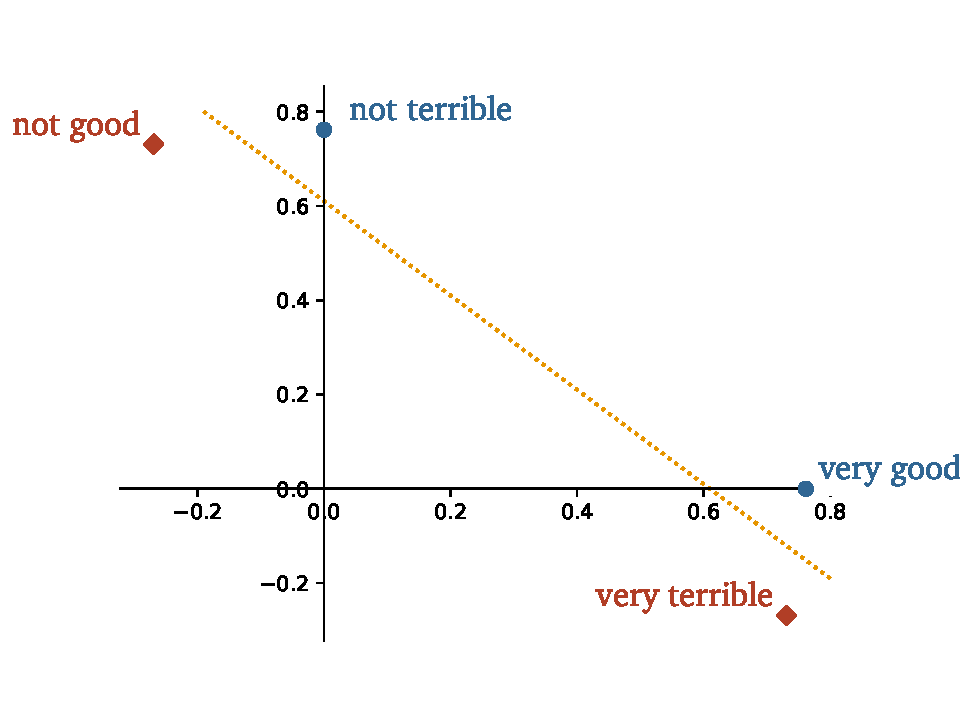
\includegraphics[width=0.9\linewidth]{./images/attention/notvery.pdf}
\end{figure}

\end{proof}

\printindex

\end{document}